%%%%%%%%%%%%%%%%%%%%%%%%%%%%%%%%%%%%%%%%%
% Masters/Doctoral Thesis
% LaTeX Template
% Version 2.5 (27/8/17)
%
% This template was downloaded from:
% http://www.LaTeXTemplates.com
%
% Version 2.x major modifications by:
% Vel (vel@latextemplates.com)
%
% This template is based on a template by:
% Steve Gunn (http://users.ecs.soton.ac.uk/srg/softwaretools/document/templates/)
% Sunil Patel (http://www.sunilpatel.co.uk/thesis-template/)
%
% Template license:
% CC BY-NC-SA 3.0 (http://creativecommons.org/licenses/by-nc-sa/3.0/)
%
%%%%%%%%%%%%%%%%%%%%%%%%%%%%%%%%%%%%%%%%%

%----------------------------------------------------------------------------------------
%	PACKAGES AND OTHER DOCUMENT CONFIGURATIONS
%----------------------------------------------------------------------------------------

% Pages (from the internal page numbering) to be printed in color - 3, 4, 5, 11, 12, 13, 14, 17, 18, 20, 21, 23, 25, 27.

\documentclass[
hidelinks,
12pt, % The default document font size, options: 10pt, 11pt, 12pt
oneside, % Two side (alternating margins) for binding by default, uncomment to switch to one side
english, % ngerman for German
doublespacing, % Single line spacing, alternatives: onehalfspacing or singlespacing
%draft, % Uncomment to enable draft mode (no pictures, no links, overfull hboxes indicated)
%nolistspacing, % If the document is onehalfspacing or doublespacing, uncomment this to set spacing in lists to single
%liststotoc, % Uncomment to add the list of figures/tables/etc to the table of contents
%toctotoc, % Uncomment to add the main table of contents to the table of contents
%parskip, % Uncomment to add space between paragraphs
%nohyperref, % Uncomment to not load the hyperref package
headsepline, % Uncomment to get a line under the header
%chapterinoneline, % Uncomment to place the chapter title next to the number on one line
%consistentlayout, % Uncomment to change the layout of the declaration, abstract and acknowledgements pages to match the default layout
]{MastersDoctoralThesis} % The class file specifying the document structure

\usepackage[utf8]{inputenc} % Required for inputting international characters
\usepackage[T1]{fontenc} % Output font encoding for international characters
\usepackage{subcaption}
\usepackage{mathpazo} % Use the Palatino font by default
%\usepackage{newpxtext,newpxmath}
\usepackage{booktabs}
\usepackage{colortbl}
\usepackage[final]{pdfpages}
\usepackage{xcolor}
\usepackage{balance}
\usepackage{epigraph}
\usepackage{alltt} % for code snippet
\usepackage{listings}
\usepackage{hyperref}
\usepackage{amsmath}
\usepackage[backend=bibtex,style=authoryear,natbib=true]{biblatex} % Use the bibtex backend with the authoryear citation style (which resembles APA)

\addbibresource{biblio.bib} % The filename of the bibliography

% Standard packages
\usepackage{amssymb,amsmath,amsthm}
\usepackage{xcolor,graphicx}
\usepackage{verbatim}
\usepackage{hyperref}
% To use turkish characters
\usepackage[utf8]{inputenc}
% Layout of headers & footers
\usepackage{titling}

% Hyphenation
\hyphenation{non-zero}

% Theorem definitions in the amsthm standard
\newtheorem{thm}{Theorem}
\newtheorem{lem}[thm]{Lemma}
\newtheorem{sublem}[thm]{Sublemma}
\newtheorem{prop}[thm]{Proposition}
\newtheorem{cor}[thm]{Corollary}
\newtheorem{conc}[thm]{Conclusion}
\newtheorem{conj}[thm]{Conjecture}
\theoremstyle{definition}
\newtheorem{defn}[thm]{Definition}
\newtheorem{cond}[thm]{Condition}
\newtheorem{asm}[thm]{Assumption}
\newtheorem{ntn}[thm]{Notation}
\newtheorem{prob}[thm]{Problem}
\theoremstyle{remark}
\newtheorem{rmk}[thm]{Remark}
\newtheorem{eg}[thm]{Example}
\newtheorem*{hint}{Hint}

%% Mathmode shortcuts
% Number sets
\newcommand{\NN}{\mathbb N}              % The set of naturals
\newcommand{\NNzero}{\NN_0}              % The set of naturals including zero
\newcommand{\NNone}{\NN}                 % The set of naturals excluding zero
\newcommand{\ZZ}{\mathbb Z}              % The set of integers
\newcommand{\QQ}{\mathbb Q}              % The set of rationals
\newcommand{\RR}{\mathbb R}              % The set of reals
\newcommand{\CC}{\mathbb C}              % The set of complex numbers
\newcommand{\KK}{\mathbb K}              % An arbitrary field
% Modern typesetting for the real and imaginary parts of a complex number
\renewcommand{\Re}{\operatorname*{Re}} \renewcommand{\Im}{\operatorname*{Im}}
% Upright d for derivatives
\newcommand{\D}{\ensuremath{\,\mathrm{d}}}

\newcommand{\Div}{\ensuremath{\,\mathrm{div}\,}}

\newcommand{\X}{\ensuremath{{\bf x}}}

\newcommand{\V}{\ensuremath{{\bf v}}}

\newcommand{\U}{\ensuremath{{\bf u}}}

\newcommand{\N}{\ensuremath{{\bf n}}}

% Upright i for imaginary unit
\newcommand{\ri}{\ensuremath{\mathrm{i}}}
% Upright e for exponentials
\newcommand{\re}{\ensuremath{\mathrm{e}}}
% abbreviation for \lambda
\newcommand{\la}{\ensuremath{\lambda}}
% Make epsilons look more different from the element symbol
\renewcommand{\epsilon}{\varepsilon}
% Always use slanted forms of \leq, \geq
\renewcommand{\geq}{\geqslant}
\renewcommand{\leq}{\leqslant}
% Shorthand for "if and only if" symbol
\newcommand{\Iff}{\ensuremath{\Leftrightarrow}}
% Make bold symbols for vectors
\providecommand{\BVec}[1]{\mathbf{#1}}
% Hyperbolic functions
\providecommand{\sech}{\operatorname{sech}}
\providecommand{\csch}{\operatorname{csch}}
\providecommand{\ctnh}{\operatorname{ctnh}}
% sinc function
\providecommand{\sinc}{\operatorname{sinc}}

% add two sub and superscripts with a space between them
\newcommand{\Mspacer}{\;} %Spacer for below Matrix display functions
\newcommand{\M}[3]{#1_{#2\Mspacer#3}} %Print a symbol with two subscripts eg a matrix entry
\newcommand{\Msup}[4]{#1_{#2\Mspacer#3}^{#4}} %Print a symbol with two subscripts and a superscript eg a matrix entry
\newcommand{\Msups}[5]{#1_{#2\Mspacer#3}^{#4\Mspacer#5}} %Print a symbol with two subscripts and two superscripts eg a matrix entry
\newcommand{\MAll}[7]{\prescript{#1}{#2}{#3}_{#4\Mspacer#5}^{#6\Mspacer#7}} %Print a symbol with two subscripts and two superscripts eg a matrix entry

% Make really wide hat for Fourier transforms applied to large functions
\usepackage{scalerel}
\usepackage{stackengine}
\stackMath
\newcommand\reallywidecheck[1]{%
\savestack{\tmpbox}{\stretchto{%
  \scaleto{%
    \scalerel*[\widthof{\ensuremath{#1}}]{\kern-.6pt\bigwedge\kern-.6pt}%
    {\rule[-\textheight/2]{1ex}{\textheight}}%WIDTH-LIMITED BIG WEDGE
  }{\textheight}% 
}{0.5ex}}%
\stackon[1pt]{#1}{\scalebox{-1}{\tmpbox}}%
}
\providecommand{\widecheck}{\reallywidecheck}

\newcommand\reallywidehat[1]{%
\savestack{\tmpbox}{\stretchto{%
  \scaleto{%
    \scalerel*[\widthof{\ensuremath{#1}}]{\kern-.6pt\bigwedge\kern-.6pt}%
    {\rule[-\textheight/2]{1ex}{\textheight}}%WIDTH-LIMITED BIG WEDGE
  }{\textheight}% 
}{0.5ex}}%
\stackon[1pt]{#1}{\tmpbox}%
}

\usepackage[autostyle=true]{csquotes} % Required to generate language-dependent quotes in the bibliography

%----------------------------------------------------------------------------------------
%	MARGIN SETTINGS
%----------------------------------------------------------------------------------------

\geometry{
	paper=a4paper, % Change to letterpaper for US letter
	inner=4.0cm, % Inner margin
	outer=3.0cm, % Outer margin
	bindingoffset=.5cm, % Binding offset
	top=2.5cm, % Top margin
	bottom=2.5cm, % Bottom margin
	%showframe, % Uncomment to show how the type block is set on the page
}

%----------------------------------------------------------------------------------------
%	THESIS INFORMATION
%----------------------------------------------------------------------------------------

\thesistitle{Approximate equations in the shallow water regime of the water wave problem on unbounded domains} % Your thesis title, this is used in the title and abstract, print it elsewhere with \ttitle
\supervisor{Pr. Katie \textsc{Oliveras}} % Your supervisor's name, this is used in the title page, print it elsewhere with \supname
\examiner{Dr/Pr. FirstName \textsc{LastName}} % Your examiner's name, this is not currently used anywhere in the template, print it elsewhere with \examname
\degree{B.Sc (Hons)} % Your degree name, this is used in the title page and abstract, print it elsewhere with \degreename
\author{Sultan \textsc{Aitzhan}} % Your name, this is used in the title page and abstract, print it elsewhere with \authorname
\addresses{} % Your address, this is not currently used anywhere in the template, print it elsewhere with \addressname

\subject{Mathematical, Computational and Statistical Sciences} % Your subject area, this is not currently used anywhere in the template, print it elsewhere with \subjectname
\keywords{Insert, keywords, here} % Keywords for your thesis, this is not currently used anywhere in the template, print it elsewhere with \keywordnames
\university{\href{https://www.yale-nus.edu.sg/}{Yale-NUS College}} % Your university's name and URL, this is used in the title page and abstract, print it elsewhere with \univname
\department{{}} % Your department's name and URL, this is used in the title page and abstract, print it elsewhere with \deptname
\group{{}} % Your research group's name and URL, this is used in the title page, print it elsewhere with \groupname
\faculty{{}} % Your faculty's name and URL, this is used in the title page and abstract, print it elsewhere with \facname

\AtBeginDocument{
\hypersetup{colorlinks=false}
\hypersetup{pdftitle=\ttitle} % Set the PDF's title to your title
\hypersetup{pdfauthor=\authorname} % Set the PDF's author to your name
\hypersetup{pdfkeywords=\keywordnames} % Set the PDF's keywords to your keywords
}

\begin{document}

\frontmatter % Use roman page numbering style (i, ii, iii, iv...) for the pre-content pages

\pagestyle{plain} % Default to the plain heading style until the thesis style is called for the body content

%----------------------------------------------------------------------------------------
%	TITLE PAGE
%----------------------------------------------------------------------------------------

\begin{titlepage}
% Fill out the titlepage.docx document, then save it as a pdf for inclusion here
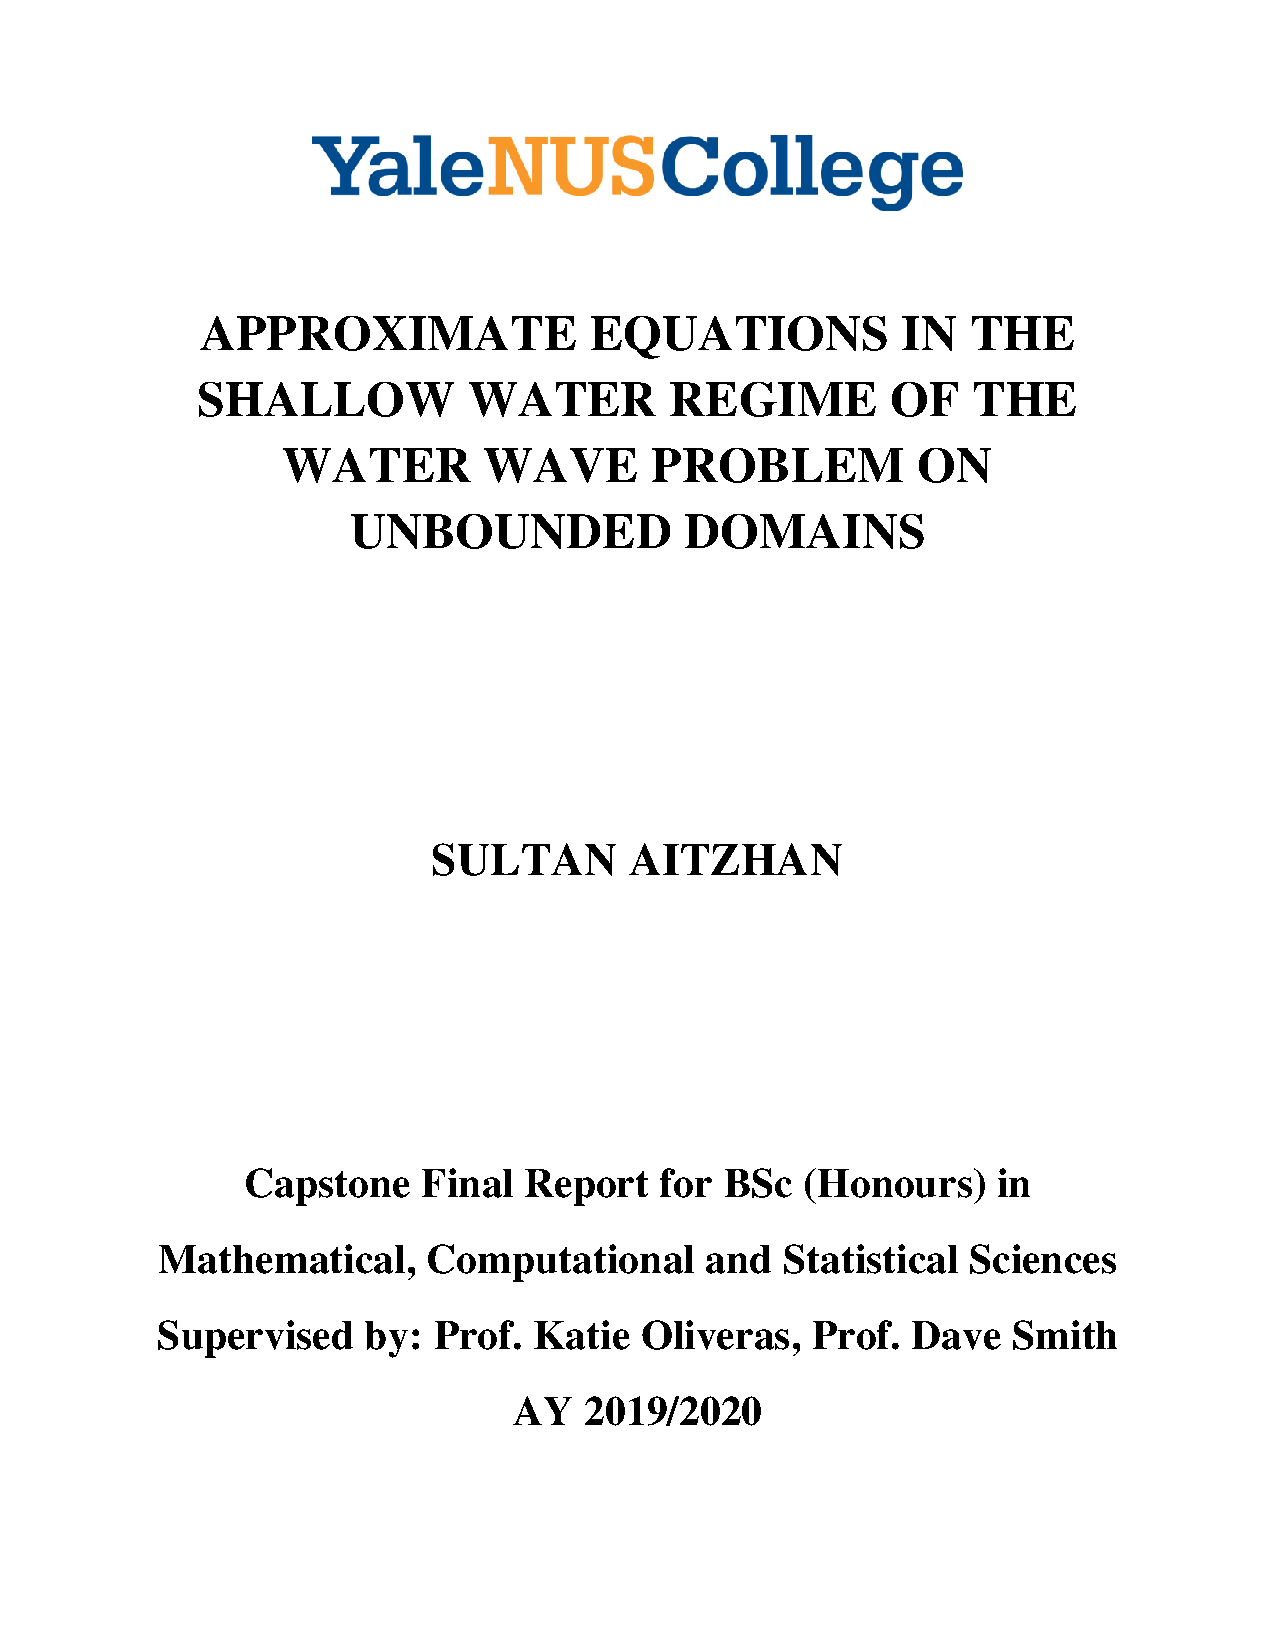
\includepdf[pages=-,pagecommand={},width=\textwidth]{titlepage.pdf}

\end{titlepage}

%----------------------------------------------------------------------------------------
%	DECLARATION & CONSENT
%----------------------------------------------------------------------------------------

% print, sign, and scan the declaration form, then include it here
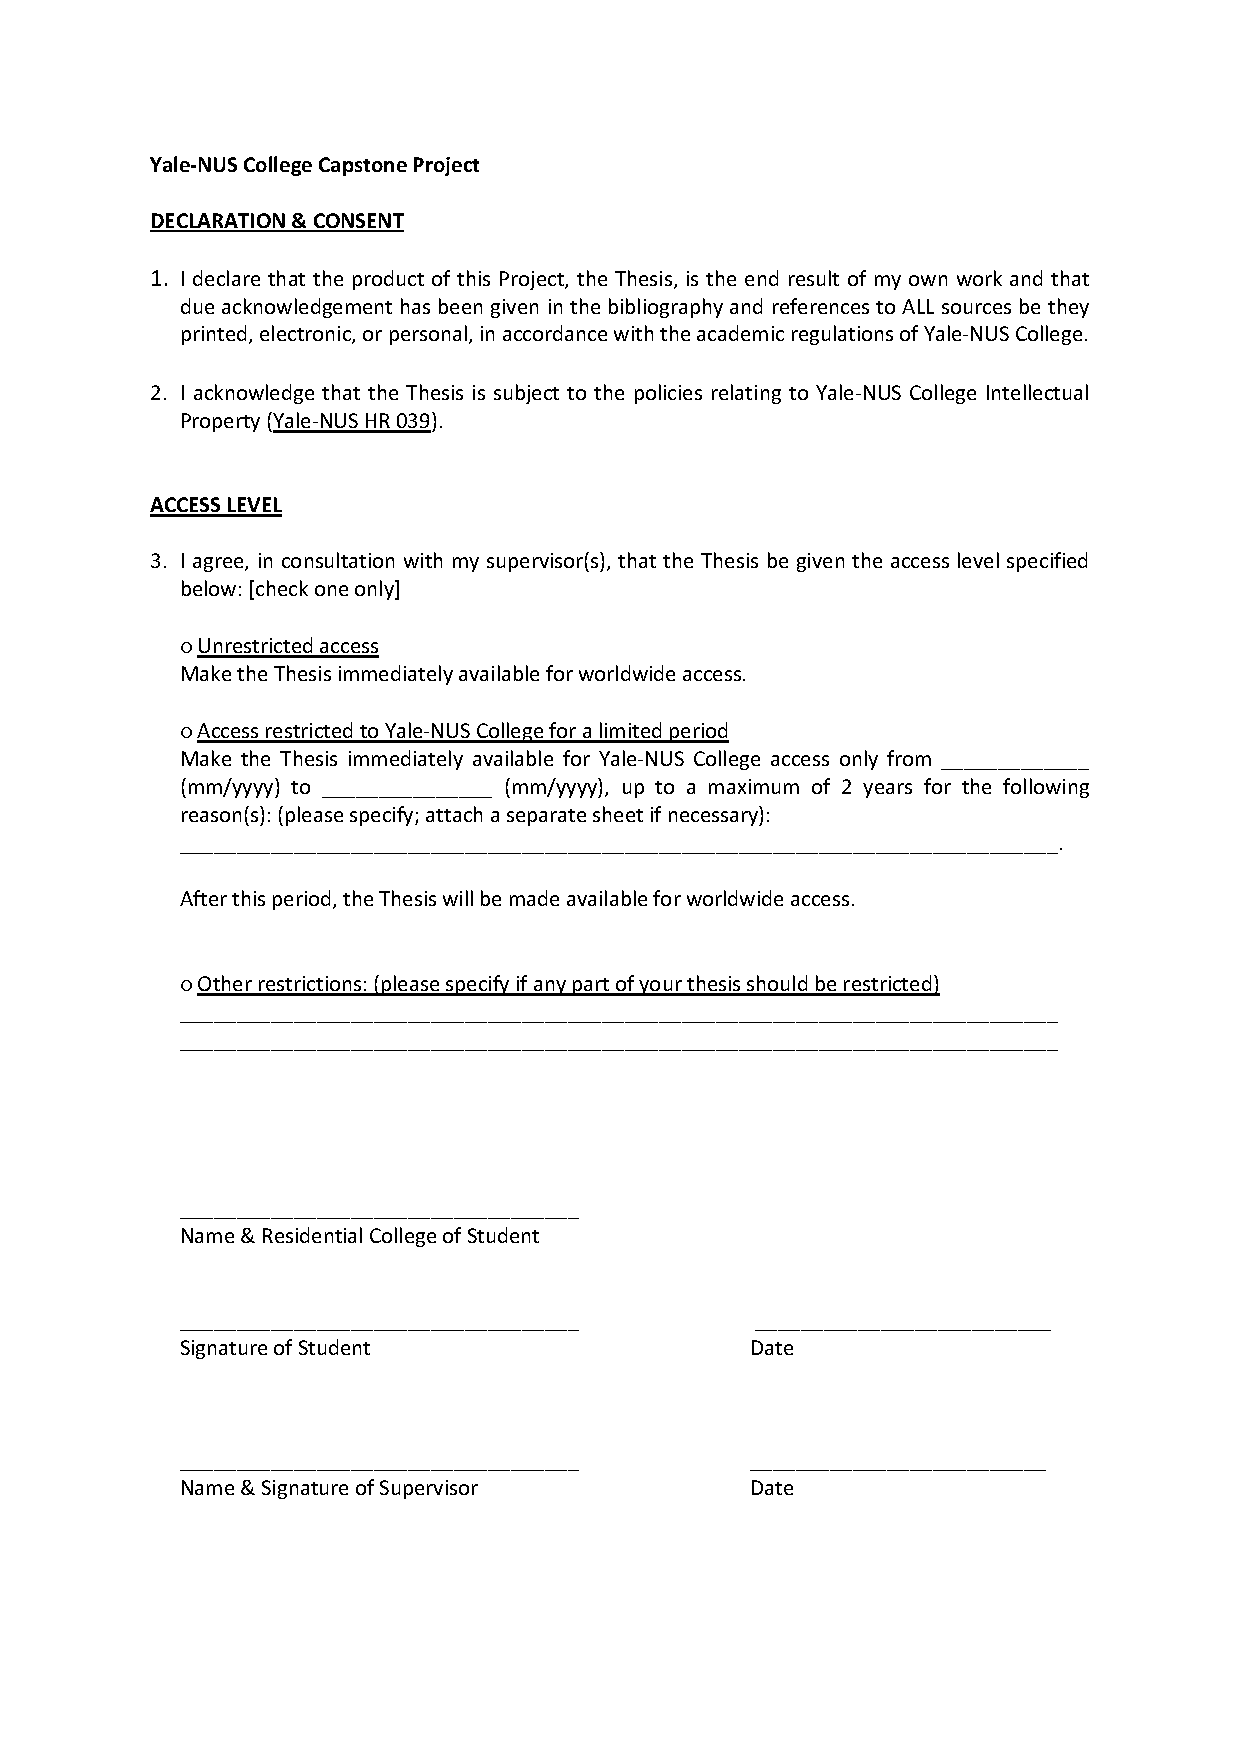
\includepdf[pages=-,pagecommand={},width=\textwidth]{declaration.pdf}

%----------------------------------------------------------------------------------------
%	ACKNOWLEDGEMENTS
%----------------------------------------------------------------------------------------

%\begin{acknowledgements}
%\addchaptertocentry{\acknowledgementname} % Add the acknowledgements to the table of contents
%Acknowledgements go here.
%\end{acknowledgements}

%----------------------------------------------------------------------------------------
%	ABSTRACT PAGE
%----------------------------------------------------------------------------------------

%\begin{abstract}
%\addchaptertocentry{\abstractname} % Add the abstract to the table of contents
%Abstract goes here.
%\end{abstract}


%----------------------------------------------------------------------------------------
% CONTRIBUTIONS
%----------------------------------------------------------------------------------------

% \chapter{Claims}
%
% This paper presents the following original contributions:
%
% \begin{enumerate}
% 	\item A hardware device for haptic sensory substitution along with designs for the construction of such a system.
% 	\item Two implementations of sensory substitution using haptic feedback, continuous and delayed feedback-based spatial navigation tasks, each of which include:
% 		\begin{enumerate}
% 			\item a front-end for providing visual input to the user during the training phase with useful readouts to the researcher,
% 			\item a transmission protocol, which maps information from the task at hand (spatial coordinates, velocity information, etc) to time-based sensor actuation signals (20$^{\circ}$ on servo 1, 35$^{\circ}$ on servo 2, etc) in real-time.
% 		\end{enumerate}
% 	\item An evaluation framework for measuring the performance of a sensory substitution system, which provides sample tasks that can be used to standardise and compare performance across the board for future research.
% 	\item A review of existing hardware and software stacks as well as possible avenues for development based on the developed metrics.
% \end{enumerate}
%
% In addition, code for displaying results in real-time, modules for managing servo overload, network latency and other factors were also written by the author.


% %----------------------------------------------------------------------------------------
% %	DECLARATION PAGE
% %----------------------------------------------------------------------------------------
%
% \begin{declaration}
% \addchaptertocentry{\authorshipname} % Add the declaration to the table of contents
%
% \noindent I, \authorname, hereby declare that this Project, the Capstone Report and associated work listed herein, is the end result of my own work and that due acknowledgement has been given in the bibliography and references to ALL sources printed, electronic, or personal, in accordance with the academic regulations of Yale‐NUS College.
% I acknowledge that the Thesis is subject to the policies relating to Yale‐NUS College Intellectual  Property (Yale‐NUS HR 039).
%
%
% % I confirm that:
% %
% % \begin{itemize}
% % \item This work was done wholly or mainly while in candidature for a research degree at this University.
% % \item Where any part of this thesis has previously been submitted for a degree or any other qualification at this University or any other institution, this has been clearly stated.
% % \item Where I have consulted the published work of others, this is always clearly attributed.
% % \item Where I have quoted from the work of others, the source is always given. With the exception of such quotations, this thesis is entirely my own work.
% % \item I have acknowledged all main sources of help.
% % \item Where the thesis is based on work done by myself jointly with others, I have made clear exactly what was done by others and what I have contributed myself.\\
% % \end{itemize}
%
% \noindent Signed:\\
% \rule[0.5em]{25em}{0.5pt} % This prints a line for the signature
%
% \noindent Date:\\
% \rule[0.5em]{25em}{0.5pt} % This prints a line to write the date
% \end{declaration}
%
% \cleardoublepage

%----------------------------------------------------------------------------------------
%	QUOTATION PAGE
%----------------------------------------------------------------------------------------

% \vspace*{0.2\textheight}
%
% \noindent\enquote{\itshape Thanks to my solid academic training, today I can write hundreds of words on virtually any topic without possessing a shred of information, which is how I got a good job in journalism.}\bigbreak
%
% \hfill Dave Barry

%----------------------------------------------------------------------------------------
%	LIST OF CONTENTS/FIGURES/TABLES PAGES
%----------------------------------------------------------------------------------------

\tableofcontents % Prints the main table of contents

%\listoftables % Prints the list of tables
%\label{lst:tabs}

%\listoffigures % Prints the list of figures
%\label{lst:figs}
%----------------------------------------------------------------------------------------
%	ABBREVIATIONS
%----------------------------------------------------------------------------------------

% \begin{abbreviations}{ll} % Include a list of abbreviations (a table of two columns)
%
% \textbf{LAH} & \textbf{L}ist \textbf{A}bbreviations \textbf{H}ere\\
% \textbf{WSF} & \textbf{W}hat (it) \textbf{S}tands \textbf{F}or\\
%
% \end{abbreviations}

%----------------------------------------------------------------------------------------
%	PHYSICAL CONSTANTS/OTHER DEFINITIONS
%----------------------------------------------------------------------------------------

% \begin{constants}{lr@{${}={}$}l} % The list of physical constants is a three column table
%
% % The \SI{}{} command is provided by the siunitx package, see its documentation for instructions on how to use it
%
% Speed of Light & $c_{0}$ & \SI{2.99792458e8}{\meter\per\second} (exact)\\
% %Constant Name & $Symbol$ & $Constant Value$ with units\\
%
% \end{constants}

%----------------------------------------------------------------------------------------
%	SYMBOLS
%----------------------------------------------------------------------------------------

% \begin{symbols}{lll} % Include a list of Symbols (a three column table)
%
% $a$ & distance & \si{\meter} \\
% $P$ & power & \si{\watt} (\si{\joule\per\second}) \\
% %Symbol & Name & Unit \\
%
% \addlinespace % Gap to separate the Roman symbols from the Greek
%
% $\omega$ & angular frequency & \si{\radian} \\
%
% \end{symbols}

%----------------------------------------------------------------------------------------
%	DEDICATION
%----------------------------------------------------------------------------------------

%\dedicatory{Dedicated to ceux l\`{a} qui veulent.}

%----------------------------------------------------------------------------------------
%	THESIS CONTENT - CHAPTERS
%----------------------------------------------------------------------------------------

\mainmatter % Begin numeric (1,2,3...) page numbering

\pagestyle{thesis} % Return the page headers back to the "thesis" style

% Include the chapters of the thesis as separate files from the Chapters folder
% Uncomment the lines as you write the chapters

% Chapter 1

\chapter{Introduction} % Main chapter title

\label{chapter1} % For referencing the chapter elsewhere, use \ref{chapter1}

Often, mathematical modelling of the real-world phenomena results in ordinary and partial differential equations, whose solutions describe the phenomena. Depending on the equations, mathematicians may or may not have the tools to obtain solutions. Fortunately, there are techniques that allow one to analyse differential equations without directly solving them. One such tool is asymptotic analysis, which leads to simplified equations that are similar to original equations. As such, solutions of the simplified equations model the real-world phenomenon, subject to some error estimates.

In particular, one problem that is amenable to asymptotic methods is the \textit{water-wave problem}, which describes the motion of water and its surface under certain conditions. Assuming an irrotational, incompressible, and inviscid fluid, and a domain with flat bottom, the equations of fluid motion are given by
\begin{subequations} \label{S1:DimWholeLineProblem}
\begin{align}
\phi_{xx} + \phi_{zz} &= 0, &-h < z < \eta(x,t), \label{S1:PDE}\\
\phi_{z} &= 0, &z = -h, \label{S1:BBC}\\
\phi_t + g\eta + \frac{1}{2}(\phi_{x}^2 + \phi_{z}^2) &= 0, &z = \eta(x,t), \label{S1:DBC} \\
\eta_t + \phi_{x}\eta_{x} &= \phi_{z}, & z = \eta(x,t), \label{S1:KBC}
\end{align}
\end{subequations}
where $\phi(x,z,t)$ is the unknown velocity potential, $\nabla \phi$ is the fluid velocity, and $\eta(x,t)$ is the unknown surface elevation. In addition, $z$ is the vertical coordinate, $x$ is the horizontal direction, and $g$ is acceleration due to gravity. We let $x\in\RR,$ so that \eqref{S1:DimWholeLineProblem} is the water-wave problem defined \textit{on the whole line}. Although nonlinear partial differential equations (PDEs) \eqref{S1:KBC} and \eqref{S1:DBC} are hard to solve on their own, what makes the problem \eqref{S1:DimWholeLineProblem} truly difficult is the need to solve the Laplace's equation \eqref{S1:PDE} on a domain with an unknown shape. 

To make the equations of motion more tractable, one can reformulate the problem and apply tools of asymptotics. Of particular interest is the work of \cite{AFM2006} (AFM formulation). In this paper, authors rewrite \eqref{S1:DimWholeLineProblem} as a system of two equations, for the surface variable $q(x,t) = \phi(x, \eta(x,t)),$ i.e. the velocity potential evaluated at the surface. Taking advantage of the new formulation, asymptotic reductions are performed in various physical conditions.

One such interesting physical condition is the shallow water regime, which is defined by small-amplitude waves that have a small depth relative to their wavelength. In this regime, asymptotic methods reveal that the fluid motion is governed by the following approximate equations: the \textit{wave} equation,
\begin{equation}\label{S1:eq1}
q_{tt} - q_{xx} = 0,
\end{equation} 
and two \textit{Korteweg de Vries (KdV)} equations,
\begin{equation}\label{S1:eq2}
\begin{aligned}
F_{T} + \frac{1}{3}F_{\xi \xi \xi} + 3 F F_{\xi} &= 0, \\
G_{T} + \frac{1}{3}G_{\zeta \zeta \zeta} + 3 G G_{\zeta} &= 0, \\
\end{aligned}
\end{equation}
where $\xi = x -t, \zeta = x+ t,$ and $q(x,t) = F(\xi, T) + G(\zeta, T).$ Physically, $F$ and $G$ can be interpreted as right-going and left going waves, respectively. The model given by \eqref{S1:eq1} and \eqref{S1:eq2} is called the \textit{KdV model on the whole line}. We observe that on \textit{the half-line}, when waves are bounded from one side by a wall, a rigorous derivation of the corresponding model remains unknown.

In this capstone project, we consider an alternative formulation of \eqref{S1:DimWholeLineProblem}, as presented in \cite{OV2013}. Although slightly different from the AFM formulation, it is contended that this formulation is well-suited for studying asymptotics. We further advocate the efficacy of this formulation by re-deriving the KdV model. 

As a brief outline, in Chapter 2, we introduce the reader to asymptotic and perturbative methods needed for the derivation. In Chapter 3, we explain the physical assumptions of the problem and describe the shallow-water regime. In Chapter 4, we reformulate the problem and derive the approximate equations.  In Chapter 5, we describe an application of the formulation to a water wave problem on \textit{the half line}, while attempting to rigorously derive a half-line model. 

% Chapter Template

\chapter{Preliminaries} % Main chapter title

\label{Chapter2} % Change X to a consecutive number; for referencing this chapter elsewhere, use \ref{ChapterX}

%----------------------------------------------------------------------------------------
%	SECTION 1
%----------------------------------------------------------------------------------------
%In this section, we present various techniques of asymptotics, explain the water wave problem in greater detail, and comment on why we can rely on asymptotics. This chapter assumes familiarity with a basic theory of ordinary and partial differential equations.

\section{Water waves problem}
In this section, a sketch of the derivation of the water wave problem will be provided, along with mathematical and physical justification of assumptions made. In addition, we discuss the shallow water limit. 

Conservation of mass \eqref{S2:CoMass} and conservation of momentum \eqref{S2:CoMomentum} are the two core principles that provide the relevant equations of fluid dynamics
\begin{align}
\frac{\partial \rho}{\partial t} + \nabla \cdot (\rho \V) &= 0, \label{S2:CoMass} \\
\rho\left[ v\frac{\partial \V}{\partial t} + (\V \cdot \nabla) \V\right] &= \textbf{F} - \nabla P + v_{\star} \Delta \V. \label{S2:CoMomentum}
\end{align}
In \eqref{S2:CoMass}-\eqref{S2:CoMomentum}, $\rho = \rho(\X, t)$ denotes the fluid mass density, $\V = \V(\X,t)$ is the fluid velocity, $P$ refers to pressure, $\textbf{F}$ is an external force, and $v_{\star}$ is the kinematic viscosity due to frictional forces. Derivations of \eqref{S2:CoMass} and \eqref{S2:CoMomentum} can be found in \cite[Chapter 3]{Johnson} or \cite[Chapter 1]{CM}. Assuming that the fluid is inviscid, incompressible, and irrotational, one can follow \cite[Section 5.1]{Ablowitz} to obtain the following system:
\begin{subequations} \label{S2:DimWholeLineProblem}
\begin{align}
\phi_{xx} + \phi_{zz} &= 0 &-h < z < \eta(x,t) \label{S2:PDE}\\
\phi_{z} &= 0 &z = -h \label{S2:BBC}\\
\eta_t + \phi_{x}\eta_{x} &= \phi_{z} & z = \eta(x,t) \label{S2:KBC}\\
\phi_t + g\eta + \frac{1}{2}(\phi_{x}^2 + \phi_{z}^2) &= 0 &z = \eta(x,t) \label{S2:DBC}
\end{align}
\end{subequations}
where $\phi(x,z)$ is the fluid velocity, $\eta(x)$ is the surface elevation. In addition, $z$ is the vertical coordinate, $x$ is the horizontal direction, and $g$ is acceleration due to gravity. In deriving the problem \eqref{S2:DimWholeLineProblem}, the following assumptions are made:
\begin{itemize}
\item We can write $\V = \nabla \phi.$
\item The problem has 1 horizontal dimension $x \in \RR.$
\item The fluid $\V$ tends to equilibrium as $|x| \to \infty.$
\item The surface tension is negligible, i.e. $\sigma = 0.$ 
\item The external force is the buoyancy force, i.e. $\textbf{F} = - \nabla (\rho_0 g z).$
\item The pressure vanishes on the surface, $P = 0$ at $z = \eta(x,t).$
\item The fluid density is constant, i.e. $\rho(\X,t) = \rho_0.$
\end{itemize}
Since the problem is expressed in terms of $\phi,$ and it is a scalar potential of velocity $\V,$ we term the formulation \eqref{S2:DimWholeLineProblem} as the \textit{velocity potential} formulation.

We begin to describe the physical meaning of the problem \eqref{S2:DimWholeLineProblem}. First, we elaborate on each equation:
\begin{itemize}
\item[\eqref{S2:PDE}:] The assumption that the fluid is irrotational means that the curl vanishes:
\[ \nabla \times \V = 0. \]
The conservation of mass then becomes $ \nabla \cdot \V = \nabla \cdot \nabla \phi = 0.$ In other words, \eqref{S2:PDE} represents that the fluid inside the domain $-h < z < \eta(x,t), x \in \RR$ does not rotate.  
\item[\eqref{S2:DBC}:] This equation is the conservation of momentum applied at the surface $z = \eta(x,t).$ Since conservation of momentum is a statement about the balance of external forces and fluid at the boundary, which is the fluid's surface, this equation describes the dynamics of the velocity potential on the free surface. As such, we term \eqref{S2:DBC} as \textit{the dynamic boundary condition}.
\item[\eqref{S2:KBC}:] This equation represents the condition that the surface $\eta$ is a surface of the fluid. In order words, we require that the surface $\eta$ is always composed of 
fluid particles that remain on the surface. We call \eqref{S2:KBC} \textit{the kinematic boundary condition}, since it is about the geometry and shape of the surface. The condition should be contrasted with the dynamic condition, which is about the interaction of forces acting at the surface. 
\item[\eqref{S2:BBC}:] This equation is an assumption that the bottom is a flat and impermeable surface, so that the fluid cannot escape through the bottom. We call \eqref{S2:BBC} \textit{the bottom condition}. 
\end{itemize}

Second, we explain the physical assumptions and considerations that led to the mathematical formulation of the problem. While mostly following \cite[Chapter 1]{Lannes}, we also expound on some of the considerations and provide additional references. For the most part, the model is the most useful in applications to oceanography \cite{?}.
\begin{itemize}
\item The fluid is assumed to be continuous. We mainly deal with behaviour on scales that are large compared to the distance between molecules that comprise the fluid. Physical quantities such as mass and velocity are thought to be spread continuously throughout the region in question; this is termed as the continuity assumption. This is important to note, since water may have discontinuities in the form of air bubbles. Whenever this happens to a significant degree, e.g. when waves break, the problem \eqref{S2:DimWholeLineProblem} is no longer valid. A microscopic description of fluids is given by the Boltzmann equation. 
\item The fluid is assumed to be incompressible and inviscid. Since the fluid under interest is water, and its density does not change both in space and time \cite{?}.This justifies homogeneity and incompressibility. In addition, water has low viscosity \cite{?}, so we can model the flow with an inviscid model. To account for viscosity, one needs to work with Navier-Stokes equations. 
\item The fluid is assumed to be irrotational. In reality, there are rotational flows, such as tornadoes. In applications, rotational effects are not important, so we do not focus on them \cite{?}. The situation is delicate when rotational flows are taken into account; in particular, the assumption $\V = \nabla \phi$ no longer holds, and the velocity formulation should be replaced with the stream-function formulation. See \cite[p.32]{Lannes} for a detailed overview.
\item We assume that the surface and the bottom of the domain can be parametrised as graphs. One may argue that neither the surface nor the bottom need to be (classical) functions; modelling overhanging waves is such example. While this is true, assuming that the surface and the bottom are functions provides the easiest setting to work in. We can extend the model by considering more general settings \cite{?}.
\item The fluid is contained in its domain. We assume that the fluid does not leak through its bottom, nor do the fluid particles leave the fluid surface. These two conditions are given by \eqref{S2:BBC} and \eqref{S2:KBC}, respectively.
\item The bottom is assumed to be flat. In reality the bottom may differ drastically. Since the degree of bed rigidity, the porosity, and the roughness all influence the fluid to varying degrees, such bottoms are also more challenging to work with. In addition, when working in the shallow water regime (explained in the next section), it is necessary to make strong assumptions on the bottom to obtain correct asymptotics. As such, we choose to deal with the simplest case of a flat bottom. For a discussion of waves over more realistic seabeds, see \cite[Chapter 9]{DD}.
\item The fluid tends to equilibrium. This is a natural condition so long as one considers infinite domains such as the whole line. It should be noted any discussion of the rate of convergence relates to the \textit{stability} theory of water waves, and is not touched upon in this project.
\item The water depth is assumed to be bounded by some nonnegative constant. In other words, we always have that $\eta - h \geq 0.$ This is a major limitation, as it excludes vanishes shorelines. However, removing this assumption is an open problem.
\item The external force is conservative. This assumption follows naturally from conservation laws for water waves. Furthermore, for water waves, the most relevant external force are a \textit{body force}, which is the force induced by an outside source and is identical for all fluid particles, and a \textit{local force}, which is the force exerted on a fluid particle by other particles. Gravitational force and pressure is one example of a body force that one needs to consider. The local force is due to friction. Since the fluid is inviscid, no local force is present. See \cite[Chapter 4]{CK} for a detailed discussion.
\item The surface tension is negligible and the surface pressure is constant. In applications to coastal oceanography, the surface tension tends to be very small \cite{?}, which justifies the assumption. Of course, surface tension is relevant when describing some smaller scale phenomena such as ripples. Since we expect no large weather variations, we can assume that locally pressure is constant. If one is to incorporate non-constant pressure and/or surface tension, the dynamic condition \eqref{S2:DBC} needs to be changed accordingly.
\item The system is two dimensional, that is, there is one spatial dimension $x$ and one vertical dimension $z.$ By ignoring the remaining dimension $y,$ we are making an assumption that the fluid is only moving in $x$ direction. In other words, we consider the special case of \textit{no transverse waves}.  Incorporating weak transverse variation leads to a generalisation of the KdV equation, the Kadomtsev-Petviashvili equation, equation (5.33) in \cite[Chapter 5]{Ablowitz}:
\begin{equation}\label{S2:KP}
\partial_x(u_t + 6uu_x + u_{xxx}) + 3 \rho u_{yy} = 0.
\end{equation}
In \eqref{S2:KP}, if $\rho = 1,$ then water waves with small surface tension are modelled, and if $\rho = -1,$ then water waves with large surface tension are modelled.
\end{itemize}
Finally, we discuss the role of initial conditions in the water waves problem. While the wave motion is expected to be initiated in some fashion, we are mainly interested in the evolution of the wave motion in many and varied situations. As such, initial conditions are not mentioned explicitly. 

\section{Asymptotic analysis and perturbation methods}
In this section, we present an introduction to perturbation theory, and its most relevant technique, namely the multiple scale analysis. The focus is on the illustration of ideas through examples, rather than rigorous justification and proofs. Examples are from Chapters 7 and 11 of \cite{BO}.

Perturbation theory is a collection of iterative techniques used for obtaining approximate solutions to problems involving a small parameter $\epsilon$. The main idea is to represent the unknown variable $f$ as a \textit{perturbation series}, which is a formal power series 
\begin{equation}\label{S2:pertubationseries}
f = f_0 + \epsilon f_1 + \epsilon^2 f_2 + \ldots.
\end{equation} 
Substituting \eqref{S2:pertubationseries} into the original problem decomposes what is a difficult problem  into many easier ones. Solving for the first $n$ terms in the series, one obtains the approximated solution 
\[f \approx f_0 + \epsilon f_1 + \ldots + \epsilon^n f_n.\]
It should be recognised that with this approach, perturbation theory is most useful when the first few problems reveal the important features of the solution and the remaining problems give only small corrections. The perturbative techniques are applied in numerous settings, including finding roots of polynomials and solving initial value problems for differential equations.

Since we deal with the differential equations, we illustrate the method with an ODE.

\eg{
Consider the following initial-value problem:
\[ y'' + y = \frac{\cos(x)}{3 + y^2}, \qquad y(0) = y\left( \frac{\pi}{2} \right) = 2. \]
}\label{S2:example}

Observe that the perturbation series obtained in Example \ref{S2:example} converges uniformly as $\epsilon \to 0.$ However, in general, one need not expect uniform convergence. A paradigmatic example is the weakly nonlinear Duffing oscillator
\begin{equation}\label{Duffing}
 y'' + y + \epsilon y^3 = 0, \qquad y(0)=1 \qquad y'(0)=0.
\end{equation}
Application of the regular perturbation series yields
\begin{equation}\label{S2:sol}
y(t) \approx y_0 + \epsilon y_1 = \cos t + \epsilon\left(\frac{1}{32} \cos 3t -\frac{1}{32} \cos t + \frac{3}{8} t \sin t\right ),
\end{equation}
which converges as $\epsilon \to 0$ for fixed $x.$ However, one must observe that the convergence is point-wise, but not uniform. Indeed, for values $t \sim 1/\epsilon$ or larger, the presence of the $t \sin t$ term in $y_1$ implies that the amplitude of oscillation grows in $t;$ we call such terms \textit{secular}. However, solutions of the Duffing oscillator are known to be bounded. In particular, this suggests that the usual perturbation expansion of $y$ is not sufficient, and that the secularity is an outcome of this misfortune.

\subsection*{Multiple scale analysis}
When ordinary perturbative methods fail to give a uniformly accurate approximation, the method of \textit{multiple scales} comes in handy. The idea behind the multiple scales is to introduce a new variable $\tau = \epsilon t.$ Physically, $\tau$ represents a longer time scale than $t$, since $\tau$ is not negligible when $t$ is of order $1/\epsilon$ or larger. Although $y(t)$ is a function of $t$ alone, through introduction of $\tau,$ $y(t)$ becomes a function of $t$ and $\tau,$ i.e $y(t, \tau).$ As such, the multiple scales looks for solutions as functions of both $t$ and $\tau,$ treating these variables independently. It must be emphasised that such treatment in two variables is rather an artifice, needed to eliminate secularities.

We illustrate the method on the Duffing oscillator. Formally, we write
\[ y(t) = Y_0(t, \tau) + \epsilon Y_1(t, \tau) + \mathcal{O}(\epsilon^2) \]
By chain rule, we have
\[ \frac{\D}{\D t} = \frac{\partial}{\partial t} + \epsilon \frac{\partial}{\partial \tau}. \]
Note
\begin{align}
\frac{\D y}{\D t} &= \frac{\partial Y_0}{\partial t} + \epsilon \left( \frac{\partial Y_0}{\partial \tau} + \frac{\partial Y_1}{\partial t} \right) + \mathcal{O}(\epsilon^2), \label{1stD} \\
\frac{\D^2 y}{\D t^2} &=\frac{\partial^2 Y_0}{\partial t^2} + \epsilon \left( 2 \frac{\partial^2 Y_0}{\partial \tau \partial t} + \frac{\partial^2 Y_1}{\partial t^2} \right) + \mathcal{O}(\epsilon^2). \label{2ndD}
\end{align}
Substituting \eqref{1stD} and \eqref{2ndD} into \eqref{Duffing} and collecting in powers of $\epsilon$ yields
\begin{align}
\frac{\partial^2 Y_0}{\partial t^2} + Y_0 &= 0, \label{S1}\\
\frac{\partial^2 Y_1}{\partial t^2} + Y_1 &= - Y_0^3 - 2 \frac{\partial^2 Y_0}{\partial \tau \partial t}. \label{S2}
\end{align}
The general solution of \eqref{S1} is 
\begin{equation}\label{S3}
Y_0(t, \tau) = A(\tau) e^{it} + A^*(\tau) e^{-it},
\end{equation}
where $A(\tau)$ is an arbitrary complex function in $\tau.$ We determine $A(\tau)$ by requiring that secular terms do not appear in $Y_1(t, \tau).$ Substitution of \eqref{S3} into \eqref{S2} gives
\begin{equation}\label{S4}
\begin{aligned}
\frac{\partial^2 Y_1}{\partial t^2} + Y_1 &=  \left(-3 A^2 A^* - 2i \frac{\D A}{\D \tau}\right) e^{it} + \left(-3 A (A^*)^2 + 2i \frac{\D A^*}{\D \tau}\right) e^{-it}\\
&- A^3 e^{3it}  - (A^*)^3 e^{-3it}.
\end{aligned}
\end{equation}
We have already seen that $e^{it}$ and $e^{-it}$ appear in the solution of \eqref{S1}, which is the homogeneous version of \eqref{S2}. Therefore, unless the coefficients of $e^{it}$ and $e^{-it}$ are zero, the solution $Y_1$ will be secular in $\tau.$  To preclude secularity, we need $A$ needs to satisfy
\begin{align*}
-3 A^2 A^* - 2i \frac{\D A}{\D \tau} &= 0, \\
-3 A (A^*)^2 + 2i \frac{\D A^*}{\D \tau} &= 0.
\end{align*}
Observe that the two equations are complex conjugate of each other, so $A(\tau)$ is not overdetermined. Solving for $A(\tau)$ along with initial conditions $y(0)=1, y'(0)=0$ yields 
\[ A(\tau) = \frac{1}{2} e^{i3\tau/8}.\]
Thus, \eqref{S3} becomes 
\[ Y_0(t, \tau) = \cos (t + \frac{3}{8}\tau).\]
Finally, using that $\tau = \epsilon t,$ we obtain the approximated solution 
\begin{equation}\label{S2:sol2}
y(t) = \cos \left[ t(1 + \epsilon\frac{3}{8})\right] + \mathcal{O}(\epsilon), \qquad \epsilon \to 0, \quad \epsilon t = \mathcal{O}(1).
\end{equation}
To conclude, we note that \eqref{S2:sol} is approximates $y$ well for $0\leq t \ll \mathcal{O}(1/\epsilon),$ while \eqref{S2:sol2} approximates over a much larger range of $t.$ 

We remark that the choice of scales $\tau = \epsilon t$ tends to be example-specific. More generally, one may choose $\tau = f(t),$ where $f$ can be any function. For example, in 
\[ y''(t) + y - \epsilon t y= 0, \qquad y(0) = 1, \qquad y'(0) = 0\]
one would use $\tau = \sqrt{\epsilon} t,$ and for
\[ y''(t)+ \omega^2(\epsilon t) y= 0,\]
one would use $\tau = \int^t \omega (\epsilon s) \D s.$

\rmk{It is important to understand the need for multiple scales. In the example of the Duffing oscillator, we could solve the problem numerically for the exact solution, or approximate the solution via multiple scales. A question arises: why use multiple scales when we can solve the differential equations numerically? 

Note that many real-world phenomena are expressed in terms of PDEs, which are much harder to solve numerically than ODEs. Due to many differences in the physical phenomena, there is no unified analytic and numerical treatment. In addition, developing numerical schemes can be very tricky, since issues such as stability, error as well as the physical conditions need to be carefully addressed to obtain an effective software. Furthermore, the cost of numerically solving PDEs can be expensive, in terms of time required to find a solution and computational power needed if the great precision is required. The latter is particularly important for real time predicting. This is another reason to prefer multiple scales. As mentioned before, multiple scales and perturbation methods, when appropriately applied, turn the original, difficult problem into many easier problems. These problems are much easier to solve, are reliable, and provide further insight into the physics of the problem.}

\section{Are asymptotic and perturbative methods reliable?}
Given the emphasis on asymptotic and perturbative methods, one is interested whether these methods provide ``reliable" solutions. Formally, how can we justify that solutions obtained from asymptotic equations converge to the solutions of the original problem? In the context of the water waves problem, we wonder if the KdV model, provided by the shallow water approximation, is ``reasonable". Of course, in asking these questions, one needs to specify the meaning of ``reliable" and ``reasonable". Following \cite{Lannes}, the validity of our asymptotic model can be understood from the following questions:
\begin{enumerate}
\item Do the solutions of the water waves problem exist on the required time scale?
\item Do the solutions of the asymptotic, KdV model exist on the same time scale?
\item Are the asymptotic solutions close to the actual solutions with the corresponding initial data? If so, how close?
\end{enumerate}
If the answer to all three questions is positive, then the asymptotic model is \textit{fully justified}. Indeed, the KdV model is fully justified (see \cite[p. 297-298]{Lannes}). However, actual proofs of the answers are involved and require advanced mathematics (see Chapter 7 and Appendix C in \cite{Lannes}). Since the mathematical justification of the KdV model is beyond the scope of the capstone project, we choose not to discuss this topic.

\section{Shallow water regime} 
For now, the problem \eqref{S2:DimWholeLineProblem} admits numerous types of water waves: short waves, long waves, intermediate waves. In particular, we have yet to specify how water wavelength relates to the water depth. As such, we first examine the \textit{dispersion relation}, to understand the relation between wave velocity and wavelength. With this in mind, we focus on the shallow water regime, characterised by small-amplitude waves that have long wavelength, relative to the water depth. In nature, tsunamis and tidal waves are examples of this regime. In coastal engineering, this regime has implications in the design of harbours and in studying estuaries and lagoons. 

First, we consider small amplitude waves, or equivalently, we assume that $|\eta| \ll 1$ and $\Vert \nabla \phi \Vert \ll 1.$ Dispersion relation is obtained by linearisation of the problem \eqref{S2:DimWholeLineProblem} around $z=0.$ More concretely, we begin by assuming the special form of the solutions
\[
\phi_s(x,z,t) = A(k,z,t) \exp(ikx) 
\]
and 
\[ 
\eta_s(x,t) = \tilde{\eta}(k,t)\exp(ikx).
\]
We then may follow Section 5.2 of \cite{Ablowitz}, to obtain the following ODE:
\[ 
\frac{\partial^2 \tilde{\eta}}{\partial t^2} + g k \tanh(k h) \tilde{\eta} = 0.
\]
Assuming that $ \tilde{\eta}(k,t) = \tilde{\eta}(k, 0) \exp(-i \omega t)$ yields the dispersion relation
\[ 
\omega^2 = g k \tanh(k h).
\]
Here, $\omega$ is a wavelength, $k$ is a wave number, and $g$ is gravity. For shallow water, the wavelength $\omega$ is much bigger than the depth $h,$ so $k$ is very small. Therefore, $kh \ll 1,$ and expansion of $\tanh(kh)$ in $kh$ leads to
\[ \omega^2 = gk(kh - \frac{(kh)^3}{3} + \ldots)  \simeq ghk^2. \]
Thus, small amplitude water waves in shallow water have wavelength $ \omega = \pm \sqrt{gh}|k|,$ or equivalently, velocity $c_0 = \sqrt{gh}.$ 

The dispersion relation allows to determine the properties of water waves that we would like to model. In particular, knowing the velocity $c_0 = \sqrt{gh}$ allows us to \textit{rescale} the problem \eqref{S2:DimWholeLineProblem}, so that the rescaled problem models shallow water waves.

In addition to admitting numerous types of water waves, the problem \eqref{S2:DimWholeLineProblem} does not specify the dimensions of the problem. Since dimensions of the problem are directly related to the units of variables (wavelength, time, height), it can be difficult to decide which terms are negligible when performing an approximation procedure. The process of \textit{non-dimensionalisation} removes the dimensions of the problem, allowing us to work with ``pure" numbers. We define dimensionless variables as follows:
\begin{equation}\label{S2:NDvar}
z = hz' \qquad x = \lambda x' \qquad t = \frac{\lambda}{c_0}t' \qquad \eta = a \eta' \qquad \phi = \frac{\lambda g a}{c_0} \phi',
\end{equation}
where $c_0 = \sqrt{gh}$ is the shallow water speed, $\lambda$ is the typical wavelength of the initial data, and $a$ is the maximum of typical amplitude of initial data. See \cite[Sections 1.3.2-1.3.3]{Lannes} for a detailed discussion of \eqref{S2:NDvar}. We further define the following parameters 
\[ \epsilon = \frac{a}{h}, \qquad \mu = \frac{h}{\lambda}.\]
Physically, $\epsilon$ is an amplitude of the water wave, while $\mu$ is a ratio of depth to a typical wavelength. Alternatively, we regard that $\epsilon$ measures nonlinearity and $\mu$ measures dispersion. Transforming the problem \eqref{S2:DimWholeLineProblem} via chain rule and dropping the primed notation yields
\begin{subequations}\label{S2:WLPND1}
\begin{align}
\label{S2:PDEND1}  \mu^2 \phi_{xx} + \phi_{zz} &= 0 &-1 <&z < \varepsilon\eta \\
\label{S2:BC1ND1} \phi_z &= 0 &z &= -1  \\ 
\label{S2:BC2ND1} \phi_{t} + \frac{\varepsilon}{2} \left(\phi_{x}^2 + \frac{1}{\mu^2}\phi_{z}^2\right) + \eta &= 0 &z &= \varepsilon\eta(x,t)\\
\label{S2:BC3ND1} \mu^2 \left[\eta_{t} + \varepsilon \phi_{x} \eta_{x}\right] &= \phi_{z} &z &= \varepsilon\eta(x,t).
\end{align}
\end{subequations}
The problem \eqref{S2:WLPND1} is a ``normalised" problem that models shallow water waves.

Observe that we have yet to make any assumptions about the parameters $\epsilon$ and $\mu,$ nor have we prescribed any relationship between the two parameters. To obtain interesting limiting equations, we make the following assumptions:
\begin{itemize}
\item Assume $\mu \ll 1.$ Recall that $\mu$ is a ratio of depth to wavelength, and in shallow water regime, we expect depth is much smaller compared to wavelength. This justifies the assumption.
\item To obtain equations that are interesting, we should balance the parameters by connecting them to each other. This is known as the Kruskal's principle of maximal balance. We elect to choose $\varepsilon = \mu^2,$ which reflects the balance of weak nonlinearity and weak dispersion.
\item From the maximal balance, it follows that $\epsilon \ll 1.$ Physically, water waves have small amplitude, and this is the first assumption used in deriving the dispersion relation.
\end{itemize}
Thus, the nondimensional problem \eqref{S2:WLPND1} becomes:
\begin{subequations}\label{S2:WLPND2}
\begin{align}
\label{S2:PDEND2}  \varepsilon\phi_{xx} + \phi_{zz} &= 0 &-1 <&z < \varepsilon\eta \\
\label{S2:BC1ND2} \phi_z &= 0 &z &= -1  \\ 
\label{S2:BC2ND2} \phi_{t} + \frac{1}{2} \left(\varepsilon\phi_{x}^2 + \phi_{z}^2\right) + \eta &= 0 &z &= \varepsilon\eta(x,t)\\
\label{S2:BC3ND2} \varepsilon\left[\eta_{t} + \varepsilon \phi_{x} \eta_{x}\right] &= \phi_{z} &z &= \varepsilon\eta(x,t).
\end{align}
\end{subequations}
Note that there is no reason not to balance in other ways, say $\varepsilon = \sqrt{\mu}.$ There are many options, and some of them will give interesting equations, while others do not lead to anything interesting. It is this assumption in the procedure that determines the relevance of to-be-derived equations.

Finally, we describe the chief result that we seek to obtain in this project. Let us assume an expansion
\[ \phi(x,z,t) = \phi_0(x,z,t) + \epsilon \phi_1(x,z,t) + \mathcal{O}(\epsilon^2).\]
Substitution of the perturbation series into \eqref{S2:PDEND2} and \eqref{S2:BC1ND2} yields that an approximation
\begin{equation}\label{S2:PS0}
\phi = A - \frac{\epsilon}{2} A_{xx}(z+1)^2 + \frac{\epsilon^2}{4!} A_{xxxx} (z+1)^4 + \mathcal{O}(\epsilon^3),
\end{equation}
where
\[ \phi_0 = A(x,t).\]
This approximation is valid in $-1<z<\epsilon \eta.$ Substitution of the series \eqref{S2:PS0} into \eqref{S2:BC2ND2} and \eqref{S2:BC3ND2}, along with appropriate manipulations yields
\begin{equation}\label{S2:PS1}
A_{tt} - A_{xx} = \epsilon\left( \frac{A_{xxxx}}{3} - 2A_x A_{xt} - A_{xx}A_t\right),
\end{equation}
valid up to $\mathcal{O}(\epsilon).$ Assume an expansion for $A:$ 
\[ A = A_0 + \epsilon A_1 + \mathcal{O}(\epsilon^2);\]
substituting this expansion into \eqref{S2:PS1} yields
\begin{equation}\label{S2:W1}
 A_{0tt} - A_{0xx} = 0.
\end{equation}
This is the wave equation, valid within $\mathcal{O}(\epsilon^0).$ The general solution is $A_0 = F(x-t) + G(x+t),$ for some general functions $F,G.$

We would like to determine the functions $F,G.$ We first observe that \eqref{S2:PS1} has secular terms: this can be shown directly via dispersion relation, or one could solve \eqref{S2:PS1} numerically and see that the solution is unbounded in time. The presence of secular terms warrants an introduction of time scales:
\[ \tau_0 = t, \qquad \tau_1 = \epsilon t.\]
We also write 
\[ 
\xi = x- \tau_0, \qquad \zeta = x + \tau_0,
\]
so that $A_0 = A_0(\xi, \zeta, \tau_1) = F(\xi, \tau_1) + G(\zeta, \tau_1).$ Via appropriate calculations, within $\mathcal{O}(\epsilon)$, we must have 
\begin{align}
2F_{\tau_1} + \frac{1}{3}F_{\xi\xi\xi} + 3 F F_\xi &= 0 \label{S2:KdV1} \\
2G_{\tau_1} - \frac{1}{3}G_{\zeta\zeta\zeta} -  3 G G_\zeta &= 0. \label{S2:KdV2}
\end{align}
In other words, we have obtained two KdV equations, \eqref{S2:KdV1} and \eqref{S2:KdV2}, for $F$ and $G,$ which determine the leading order solution $A_0$ of the problem. 

The wave and KdV equations are special PDEs. The wave equation arises as a model in numerous fields of classical physics, such as electrodynamics, plasma physics, and general relativity. The KdV equation appears whenever long waves propagate over dispersive medium, be it fluid mechanics, nonlinear optics, or Bose-Einstein condensation. Because of how they occur independently of the applications, wave and KdV have been studied extensively. Furthermore, KdV is special: despite being nonlinear, this PDE can be solved exactly, by means of inverse scattering transform. 

In conclusion, the leading order solution of the water wave problem for small-amplitude, shallow water waves is described by the wave equation \eqref{S2:W1} and two KdV equations \eqref{S2:KdV1}, \eqref{S2:KdV2}. This is the result we seek to obtain. 
% Chapter Template

\chapter{Water-wave problem} % Main chapter title

\label{chapter3} % Change X to a consecutive number; for referencing this chapter elsewhere, use \ref{ChapterX}

%----------------------------------------------------------------------------------------
%	SECTION 1
%----------------------------------------------------------------------------------------

The theory of water waves has been a source of intriguing and difficult mathematical problems. Derived by Euler in 1757 (\cite{C2004}), the incompressible Euler equations with a free boundary, also known as the full water-wave problem, are widely regarded as the governing equations for water waves and have been the subject of extensive research. At first, the essential character of studying water waves was in bringing together equations of fluid mechanics, illustrating wave propagation, and highlighting the role of boundary conditions. However, during the last 60 years, the complexity of mathematical theories for water waves has exploded. The emergence of \textit{soliton} theory, itself conceived in the context of water waves, has transformed many mathematical aspects of nonlinear wave propagation. Today, the study of water waves is an important part of applied mathematics, serving as a diverse intersection in which many seemingly disparate parts of mathematics come together.

That water waves are a physical phenomenon has an added advantage: often, they may be analysed by direct observation. Indeed, mathematical results provide a description that can be tested whenever an expanse of water is at hand: a river, the ocean, or simply the household sink. In particular, such results may have wide-ranging implications in engineering and climate modelling. Conversely, numerical simulations by themselves have led to many advances in water waves. The complexity and variety of water-wave phenomena inform many applications but also invite other sciences to contribute, thereby making  the field suitable for multidisciplinary collaborations.

In this chapter, we delve into the water-wave problem. First, we explain the problem in greater detail and present the shallow water regime. Using asymptotic tools, we then describe and justify the derivation of the KdV model.

\section{Describing the water-wave problem}

Conservation of mass \eqref{S2:CoMass} and conservation of momentum \eqref{S2:CoMomentum} are the two core principles that provide the relevant equations of fluid dynamics. The resulting equations are 
\begin{align}
\frac{\partial \rho}{\partial t} + \nabla \cdot (\rho \V) &= 0, \label{S2:CoMass} \\
\rho\left[ v\frac{\partial \V}{\partial t} + (\V \cdot \nabla) \V\right] &= \textbf{F} - \nabla P + v_{\star} \Delta \V, \label{S2:CoMomentum}
\end{align}
where $\rho = \rho(\X, t)$ denotes the fluid mass density, $\V = \V(\X,t)$ is the fluid velocity, $P(\X, t)$ refers to pressure, $\textbf{F}(\X)$ is an external force, and $v_{\star}$ is the viscosity due to frictional forces. Derivations of \eqref{S2:CoMass} and \eqref{S2:CoMomentum} can be found in \cite[Chapter 1]{Johnson}. Assuming that the fluid is inviscid, incompressible, and irrotational, one can follow Section 5.1 of \cite{Ablowitz} to obtain the system
\begin{subequations} \label{S2:DimWholeLineProblem}
\begin{align}
\phi_{xx} + \phi_{zz} &= 0, &-h < z &< \eta(x,t), \label{S2:PDE}\\
\phi_{z} &= 0, &z &= -h, \label{S2:BBC}\\
\phi_t + g\eta + \frac{1}{2}(\phi_{x}^2 + \phi_{z}^2) &= 0, &z &= \eta(x,t), \label{S2:DBC}\\
\eta_t + \phi_{x}\eta_{x} &= \phi_{z}, &z &= \eta(x,t), \label{S2:KBC}
\end{align}
\end{subequations}
where $\phi(x,z, t)$ is a scalar field such that $\V = \nabla \phi$ and $\eta(x,t)$ is the surface elevation. In addition, $z$ is the vertical coordinate, $x$ is the horizontal direction, and $g$ is acceleration due to gravity. See Figure \ref{fig:waterwaveproblem} for a visual representation of the domain, which we denote $S = \RR \times (-h, \eta).$ In deriving \eqref{S2:DimWholeLineProblem}, the following assumptions are made:
\begin{itemize}
\item The problem has 1 horizontal dimension $x \in \RR.$
\item The fluid velocity $\V$ tends to equilibrium as $|x| \to \infty.$
\item The external force is the buoyancy due to gravity, i.e. $\textbf{F} = - \nabla (\rho_0 g z).$
\item The pressure vanishes on the surface, $P = 0$ at $z = \eta(x,t).$
\item The fluid density is constant, i.e. $\rho(\X,t) = \rho_0.$
\end{itemize}
As the problem is expressed in terms of $\phi,$ the scalar potential of velocity $\V,$ \eqref{S2:DimWholeLineProblem} is called the \textit{velocity potential} formulation of the water-wave problem.
\begin{figure}[h]
\captionsetup{width=\textwidth}
\centering
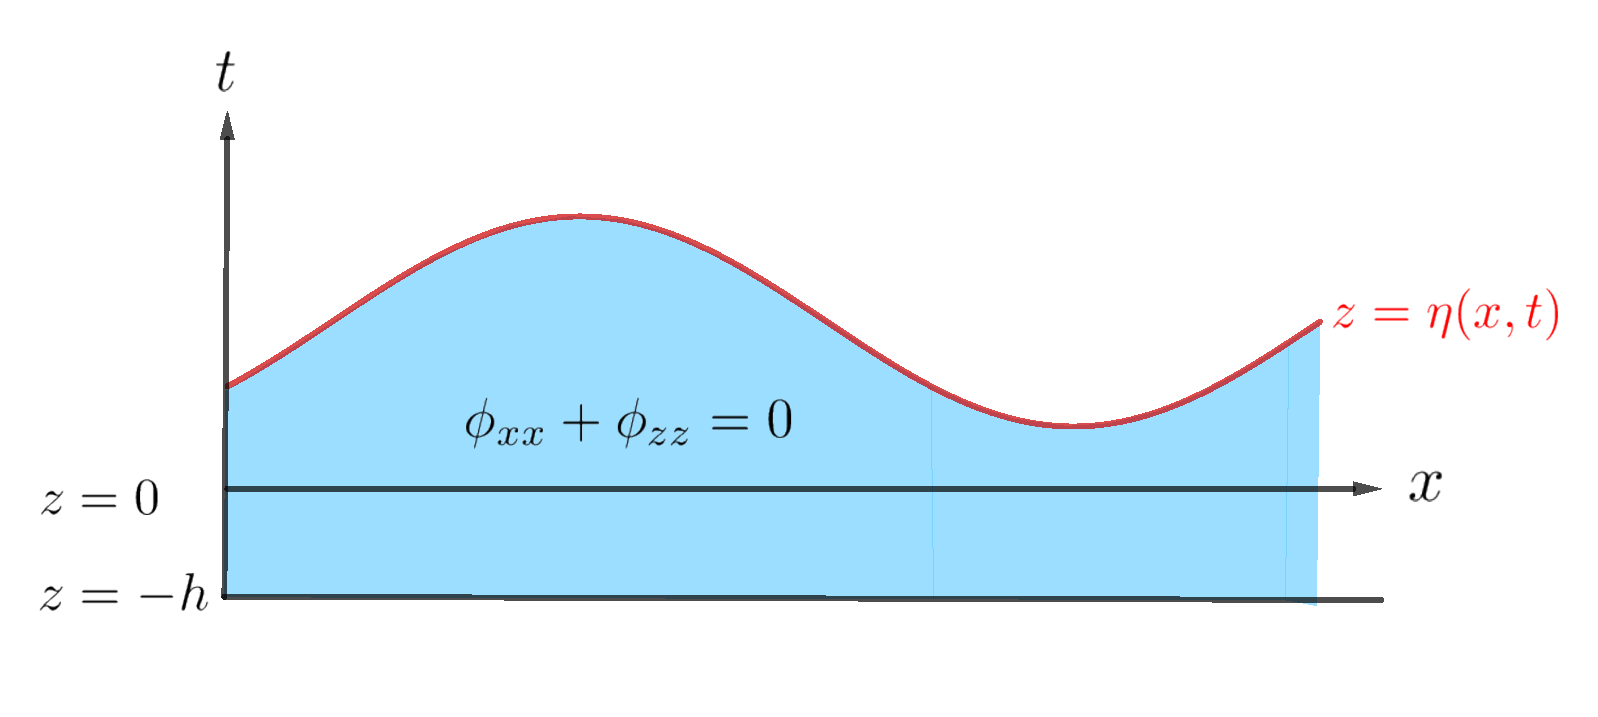
\includegraphics[width=\linewidth]{figures/waterwaveproblem.pdf}
\caption{Schematic for the domain of the water wave problem \eqref{S2:DimWholeLineProblem}.}
\label{fig:waterwaveproblem}
\end{figure}

We now describe the physical relevance of \eqref{S2:DimWholeLineProblem}, by explaining each equation:
\begin{itemize}
\item[\eqref{S2:PDE}:] Assuming that the fluid is irrotational means that the curl vanishes: $\nabla \times \V = 0.$ Thus, there is a scalar field $\phi$ such that $\nabla \phi = \V.$ Conservation of mass \eqref{S2:CoMass} then becomes $\Delta \phi = 0.$ In other words, the fluid inside the domain $S$ is incompressible and irrotational.
\item[\eqref{S2:BBC}:] This equation is an assumption that the bottom is a flat and impermeable surface, so that the fluid cannot escape through the bottom. Since $\phi_z$ is the vertical velocity, \eqref{S2:BBC} means that there is no flow through the bottom. We call \eqref{S2:BBC} \textit{the bottom condition}. 
\item[\eqref{S2:DBC}:] This equation is the conservation of momentum \eqref{S2:CoMomentum} applied at the surface $z = \eta(x,t).$ Since the conservation of momentum is a statement about the balance of external forces and fluid at the fluid's surface, this equation describes the dynamics of the velocity potential on the boundary. We call \eqref{S2:DBC} \textit{the dynamic boundary condition}.
\item[\eqref{S2:KBC}:] This equation represents the condition that $\eta$ is the surface of the fluid. In other words, the surface $z = \eta(x,t)$ is always composed of fluid particles that remain on the surface. We call \eqref{S2:KBC} \textit{the kinematic boundary condition}, since it describes the geometry and shape of the surface. The condition should be contrasted with the dynamic condition, which is about the interaction of forces acting at the surface. 
\end{itemize}

%Second, we explain some of the physical assumptions and considerations leading to the mathematical formulation of the problem. %While mostly following \cite[Chapter 1]{Lannes}, we also expound on some points and provide additional references. 
%Roughly speaking, the model is useful in applications to coastal oceanography, specifically in modelling tsunamis \cite{}.
%\begin{itemize}
%\item The fluid is assumed to be continuous. %We mainly deal with behaviour on scales that are large compared to the distance between molecules that comprise the fluid. 
%Physical quantities such as mass and velocity are spread continuously throughout the region; this is \textit{the continuity assumption}. %This is important to note, since water may have discontinuities in the form of air bubbles. Whenever this happens to a significant degree, e.g. when waves break, the problem \eqref{S2:DimWholeLineProblem} is no longer valid. A microscopic description of fluids is given by the Newton's laws and Boltzmann equation (see \cite{G2019} for a survey). 
%\item The fluid is assumed to be incompressible and inviscid. The fluid under study is pure water: its density does not change both in space and time, and it is mostly inviscid (see \cite[Appendix A2]{CK}). %One can extend the problem to work with compressible fluids. However, to account for viscosity, one needs to work with Navier-Stokes equations (see \cite[Section 1.3]{CM}. 
%\item The fluid is assumed to be irrotational. In applications considered here (e.g. tsunamis), rotational effects contribute little. %In reality, when the scales are much larger, rotational flows give rise to tornadoes, vortices and eddies. The situation is delicate when rotating effects are considered: the assumption $\V = \nabla \phi$ no longer holds, and the velocity formulation is replaced with the stream-function formulation. See \cite[p.32-35]{Lannes} for a detailed overview.
%\item The bottom is assumed to be flat. %In reality the bottom may differ drastically. Since the degree of bed rigidity, the porosity, and the roughness all influence the fluid to varying degrees, it is also more challenging to work with such bottoms. In addition, when working in the shallow water regime (as explained in the next section), it is necessary to make strong assumptions on the bottom to obtain correct asymptotics. As such, we choose to deal with the simplest case of a flat bottom. For a discussion of waves over more realistic seabeds, see \cite[Chapter 9]{DD}.
%\item We assume that the surface and the bottom of the domain can be parametrised as graphs. Neither the surface nor the bottom need to be functions; indeed, modelling overhanging waves is one such example. While this is true, assuming that the surface and the bottom are functions provides an easier setting to work in. 
%\item The fluid is contained in its domain. We assume that the fluid does not leak through its bottom, nor do the fluid particles leave the fluid surface. %These two conditions are given by \eqref{S2:BBC} and \eqref{S2:KBC}, respectively.
%%\item The fluid tends to equilibrium. This is a natural condition so long as one considers infinite domains such as the whole line. Note that any discussion of the rate of convergence relates to the \textit{stability} theory of water waves, and is not touched upon in this project.
%\item The water depth is assumed to be nonnegative. In other words, we have that $\eta - h > 0$ (see Figure \ref{fig:vanishingdepth}). %This is a major limitation, as it excludes vanishes shorelines. However, removing this assumption is an open problem. As the depth is vanishing, the size of computational domain becomes part of the solution $\phi.$ This issue leads to theoretical and numerical difficulties in describing the shoreline. There are some models that are extended to this case, though they are limited to one dimension and are not rigorously justified (see \cite{BCLMT2011}).
%\item The external force is conservative. This assumption follows naturally from conservation laws for water waves. %For our problem, relevant external forces are a \textit{body force}, which is the force due to an outside source and is identical for all fluid particles, and a \textit{local force}, which is the force exerted on a fluid particle by other particles. For our problem, gravity and pressure are pertinent body forces, and friction is the local force. Since the fluid is inviscid, no local force is present. See \cite[Chapter 4]{CK} for a detailed discussion.
%%\item The surface tension is negligible and the surface pressure is constant. In applications to coastal oceanography, the surface tension tends to be very small, which justifies the assumption (see \cite[Example 9.1, Chapter 9]{Lannes}). Since we expect no large weather variations, we can also assume that locally pressure is constant. Of course, surface tension is relevant when describing some smaller scale phenomena such as ripples. If one is to incorporate non-constant pressure and/or surface tension, the dynamic condition \eqref{S2:DBC} needs to be changed accordingly.
%%\item The system is two dimensional: there is one spatial dimension $x$ and one vertical dimension $z.$ By ignoring the remaining dimension $y,$ we assume that the fluid is moving in $x$ direction only. In other words, we consider the special case of \textit{no transverse waves}.  Incorporating weak transverse variation leads to a generalisation of the KdV equation, the Kadomtsev-Petviashvili equation:
%%\begin{equation}\label{S2:KP}
%%\partial_x(u_t + 6uu_x + u_{xxx}) + 3 \rho u_{yy} = 0.
%%\end{equation}
%%In \eqref{S2:KP}, if $\rho = 1,$ then water waves with small surface tension are modelled, and if $\rho = -1,$ then water waves with large surface tension are modelled.
%\end{itemize}
\rmk{While the wave motion is expected to be initiated in some fashion, we are mainly interested in evolution of wave motion. As such, initial conditions are not explicitly discussed.}

%\begin{figure}[h]
%\captionsetup{width=\textwidth}
%\centering
%    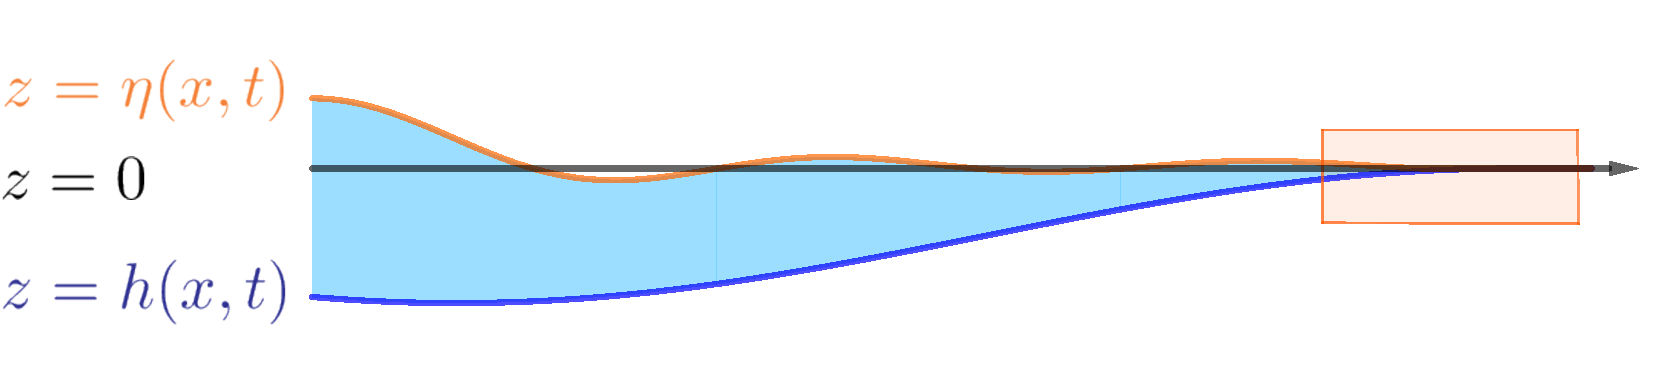
\includegraphics[width=\linewidth]{figures/vanishingdepth2.pdf}
%  \caption{The region in orange is the zone of vanishing water depth. In this region, the domain becomes part of the solution, which complicates the problem. Therefore, the problem \eqref{S2:DimWholeLineProblem} is valid in the zone to the left of the orange region.}
%  \label{fig:vanishingdepth}
%\end{figure}

\section{Shallow water regime} 
For now, \eqref{S2:DimWholeLineProblem} admits numerous types of water waves: short waves, long waves, intermediate waves. This is because we have yet to specify how wavelength relates to the water depth. Thus, we first examine the \textit{dispersion relation}, which describes the relation between wave velocity and wavelength. This will allow us to focus on the shallow water regime.

We consider small-amplitude waves, or equivalently, we assume that $|\eta| \ll 1$ and $\Vert \nabla \phi \Vert \ll 1.$ The dispersion relation is obtained by linearising the problem \eqref{S2:DimWholeLineProblem} around $z=0.$ More concretely, let $\phi_s(x,z,t) = \tilde{\phi}(k,z,t) \exp(ikx),$ and $\eta_s(x,t) = \tilde{\eta}(k,t)\exp(ikx);$ we think of $\phi_s$ and $\eta_s$ as special form solutions $\phi$ and $\eta.$ We then may follow Section 5.2 of \cite{Ablowitz}, to obtain the following ODE:
\[ 
\frac{\partial^2 \tilde{\eta}}{\partial t^2} + g k \tanh(k h) \tilde{\eta} = 0.
\]
Assuming that $\tilde{\eta}(k,t) = \tilde{\eta}(k, 0) \exp(-i \omega t),$ the above equation yields the dispersion relation $\omega^2 = g k \tanh(k h).$ Here, $\omega$ is a frequency, $k$ is a wave number, and $g$ is gravity. 

With this in mind, we focus on the shallow water regime, characterised by small-amplitude waves that have long wavelength relative to the water depth. For shallow water, the wavelength $\dfrac{2 \pi}k{}$ is much bigger than the depth $h,$ so $kh \ll 1.$ Expansion of $\tanh(kh)$ in $kh$ allows to rewrite the dispersion relation as
\[ \omega^2 = gk(kh - \frac{(kh)^3}{3} + \mathcal{O}((kh)^5))  \simeq ghk^2. \]
Thus, small-amplitude waves in shallow water have frequency $ \omega = \pm \sqrt{gh}|k|,$ or equivalently, velocity $c_0 = \sqrt{gh}.$ Now, using the dispersion relation, we can \textit{rescale} the problem \eqref{S2:DimWholeLineProblem} to model shallow water waves with velocity $c_0 = \sqrt{gh}.$ In nature, tsunamis and tidal waves are examples of this regime. 

In addition, the problem \eqref{S2:DimWholeLineProblem} does not specify the physical dimensions. Since dimensions of the problem are directly related to the units of variables such as wavelength, time, or height, it can be difficult to decide which terms are negligible when performing asymptotic reductions. The process of \textit{non-dimensionalisation} removes the physical dimensions, allowing us to work with "pure" numbers. Letting primes denote the dimensionless variables, we introduce
\begin{equation}\label{S2:NDvar}
z = hz' \qquad x = \lambda x' \qquad t = \frac{\lambda}{c_0}t' \qquad \eta = a \eta' \qquad \phi = \frac{\lambda g a}{c_0} \phi',
\end{equation}
where $c_0 = \sqrt{gh}$ is the shallow water speed, $\lambda$ is the wavelength and $a$ is the maximum amplitude of initial data. See Sections 1.3.2-1.3.3 of \cite{Lannes} for a detailed discussion of \eqref{S2:NDvar}. 

We define parameters $\epsilon = \dfrac{a}{h}, \mu = \dfrac{h}{\lambda}.$ Physically, $\epsilon$ is an amplitude of a wave relative to depth, while $\mu$ is a ratio of depth to a typical wavelength. Alternatively, we understand that $\epsilon$ measures nonlinearity and $\mu$ measures dispersion. 
%Transforming \eqref{S2:DimWholeLineProblem} via chain rule and dropping the primed notation yields 
%\begin{subequations}\label{S2:WLPND1}
%\begin{align}
%\mu^2 \phi_{xx} + \phi_{zz} &= 0, &-1 < z &< \varepsilon\eta, \label{S2:PDEND1} \\
%\phi_z &= 0, &z &= -1, \label{S2:BC1ND1} \\ 
%\phi_{t} + \frac{\varepsilon}{2} \left(\phi_{x}^2 + \frac{1}{\mu^2}\phi_{z}^2\right) + \eta &= 0, &z &= \varepsilon\eta(x,t), \label{S2:BC2ND1} \\
%\mu^2 \left[\eta_{t} + \varepsilon \phi_{x} \eta_{x}\right] &= \phi_{z}, &z &= \varepsilon\eta(x,t). \label{S2:BC3ND1} 
%\end{align}
%\end{subequations}
%The problem \eqref{S2:WLPND1} is a "normalised" problem that models shallow water waves.

Note that we have yet to make any assumptions about $\epsilon$ and $\mu,$ nor is any relationship between the two parameters prescribed. We make the following assumptions:
\begin{itemize}
\item Assume $\mu \ll 1.$ Recall that $\mu$ is a ratio of depth to wavelength, and in shallow water regime, we expect that depth is much smaller compared to wavelength.
\item To obtain interesting approximate equations, we should balance the parameters by connecting them to each other. This is \textit{the principle of maximal balance} (see \cite{Kruskal1963}). We choose $\varepsilon = \mu^2,$ which reflects the balance of weak nonlinearity and weak dispersion.
\item From the maximal balance principle, we have $\epsilon \ll 1.$ Physically, we consider water waves whose amplitude is small relative to depth.
\end{itemize}
Transforming \eqref{S2:DimWholeLineProblem} via chain rule and dropping the primed notation yields 
\begin{subequations}\label{S2:WLPND2}
\begin{align}
\label{S2:PDEND2}  \varepsilon\phi_{xx} + \phi_{zz} &= 0, &-1 <z &< \varepsilon\eta, \\
\label{S2:BC1ND2} \phi_z &= 0, &z &= -1,  \\ 
\label{S2:BC2ND2} \phi_{t} + \frac{1}{2} \left(\varepsilon\phi_{x}^2 + \phi_{z}^2\right) + \eta &= 0, &z &= \varepsilon\eta(x,t),\\
\label{S2:BC3ND2} \varepsilon\left[\eta_{t} + \varepsilon \phi_{x} \eta_{x}\right] &= \phi_{z}, &z &= \varepsilon\eta(x,t).
\end{align}
\end{subequations}
The problem \eqref{S2:WLPND2} is a "normalised" problem that models small-amplitude shallow water waves.

\rmk{
Note that there is no reason not to balance in other ways, say $\varepsilon = \sqrt{\mu}.$ There are many options: some lead to interesting equations, while others do not. Indeed, it is this assumption in the procedure that determines the relevance of the model derived below.}

\section{Deriving the KdV model}
The presence of $\epsilon$ in \eqref{S2:WLPND2} indicates that we can further simplify the problem using ideas developed in Chapter 2. Expanding $\phi(x,z,t) = \phi_0(x,z,t) + \epsilon \phi_1(x,z,t) + \mathcal{O}(\epsilon^2)$ and substituting the series into \eqref{S2:PDEND2} and \eqref{S2:BC1ND2} yields
\begin{equation}\label{S2:PS0}
\phi = A - \frac{\epsilon}{2} A_{xx}(z+1)^2 + \frac{\epsilon^2}{4!} A_{xxxx} (z+1)^4 + \mathcal{O}(\epsilon^3)
\end{equation}
valid in $-1<z<\epsilon \eta,$ where $\phi_0 = A(x,t).$ Substituting \eqref{S2:PS0} into \eqref{S2:BC2ND2} and \eqref{S2:BC3ND2}, along with appropriate manipulations, gives
\begin{equation}\label{S2:PS1}
A_{tt} - A_{xx} = \epsilon\left( \frac{A_{xxxx}}{3} - 2A_x A_{xt} - A_{xx}A_t\right),
\end{equation}
valid up to $\mathcal{O}(\epsilon).$ Obtaining \eqref{S2:PS1} is an especially lengthy calculation, since the dynamic and kinematic conditions must be expanded carefully. 

Now, we sketch out the derivation of the KdV model. Expanding $A = A_0 + \epsilon A_1 + \mathcal{O}(\epsilon^2)$ and substituting this expansion into \eqref{S2:PS1}, we have 
\begin{equation}\label{S2:W1}
\mathcal{O}(\epsilon^0): \quad A_{0tt} - A_{0xx} = 0.
\end{equation} 
This is the wave equation, whose general solution is $A_0 = F(x-t) + G(x+t),$ for some functions $F,G.$

We would like to determine $F,G.$ First, we observe that in parallel to the Duffing oscillator, \eqref{S2:PS1} contains secularities in $t$ when solving the next order euqation. %, or one could solve \eqref{S2:PS1} numerically and see that the solution is unbounded in time.
This can partly be shown via the dispersion relation and therefore an introduction of multiple time scales: $\tau_0 = t, \tau_1 = \epsilon t.$ We also let $\xi = x- \tau_0$ and $\zeta = x + \tau_0,$ so that $A_0 =  F(\xi, \tau_1) + G(\zeta, \tau_1).$ Via appropriate calculations, from \eqref{S2:PS1} one obtains 
\begin{align}
2F_{\tau_1} + \frac{1}{3}F_{\xi\xi\xi} + 3 F F_\xi &= 0, \label{S2:KdV1} \\
2G_{\tau_1} - \frac{1}{3}G_{\zeta\zeta\zeta} -  3 G G_\zeta &= 0. \label{S2:KdV2}
\end{align}
Hence, we obtain two KdV equations, \eqref{S2:KdV1} and \eqref{S2:KdV2}, which determine the dependence of $F, G$ on $\tau_1.$ Solving the KdV equations via initial conditions, we determine $\phi_0 = A_0,$ and therefore $\phi$ in the leading order.

The wave and KdV equations are well-known PDEs. The wave equation arises as a model in numerous fields of physics, such as electrodynamics, plasma physics, and general relativity. The KdV equation appears whenever long waves propagate over dispersive media, be it in the fields of fluid mechanics, nonlinear optics, or Bose-Einstein condensates. Because of how they occur independently of applications, the two equations have been studied extensively. Furthermore, the KdV equation is special: despite being nonlinear, it can be solved exactly in certain domains, using advanced techniques such as the inverse scattering transform (see Chapter 9 of \cite{Ablowitz}).

In conclusion, the leading order solution of the water wave problem for small-amplitude, shallow water waves is described by the wave equation \eqref{S2:W1} and two KdV equations \eqref{S2:KdV1}, \eqref{S2:KdV2}. This is the result we seek to obtain on the whole line using a different formulation of the problem, as well as a new extension to the half-line.

\section{Are asymptotic methods reliable?}
Given the emphasis on asymptotic and perturbative methods, one is interested whether these methods provide "reliable" solutions. Formally, how can we justify that solutions of asymptotic equations converge to solutions of the original problem? In the context of the water-wave problem \eqref{S2:DimWholeLineProblem}, is the KdV model, provided by the shallow water approximation, "reasonable"? Of course, in asking these questions, one needs to specify the meaning of ``reliable" and ``reasonable". Following \cite{Lannes}, the validity of the KdV model can be understood from the following questions:
\begin{enumerate}
\item Do the solutions of \eqref{S2:DimWholeLineProblem} exist on the required time scale?
\item Do the solutions of the KdV model exist on the same time scale?
\item Are the asymptotic solutions close to the actual solutions with the corresponding initial data? If so, how close?
\end{enumerate}
If the answer to all three questions is positive, then the asymptotic model is \textit{fully justified}. Indeed, the KdV model is fully justified (see \cite[p. 297-298]{Lannes}). The detailed proofs require advanced mathematics such as working in Sobolev spaces and applying Poincaré and Gagliardo-Nirenberg inequalities. Since the rigorous mathematical justification of the KdV model is beyond the scope of the project, we choose not to discuss this topic here, and refer the reader to Chapter 7 and Appendix C of \cite{Lannes} for the details.
% Chapter Template

\chapter{Non-local derivation on the whole line} % Main chapter title

\label{Chapter4} % Change X to a consecutive number; for referencing this chapter elsewhere, use \ref{ChapterX}

As mentioned in Chapter 3, a direct derivation of the KdV model is subject to lengthy calculations and careful bookkeeping. If we are to change domains (say, the half-line), then additional care must be taken to ensure that the model is correct. As such, we look for a more efficient way of deriving asymptotic models valid on various domains.
 
% In addition, these complications lead to difficulties when attempting to deal with questions of existence and well-posedness. 
Recall that the water-wave problem is challenging to work with directly, due to the nonlinear boundary conditions and the domain with an unknown shape. To address these issues, reformulations of the problem are introduced, which result in equivalent problems that are more tractable. Below, we give a short overview of these formulations.

For one-dimensional surfaces (one horizontal variable), conformal mappings can be used to eliminate some of the issues (for an overview, see \cite{DKSZ1996}). However, this approach is limited to one-dimensional surfaces. For both one- and two-dimensional surfaces, formulations such as the Hamiltonian formulation given in \cite{Zakharov} or \cite{CS1993} reduce the problem to a system of two equations in terms of surface variables $q(x,t) = \phi(x, \eta(x,t),t)$ and $\eta(x,t).$ This is achieved by introducing a Dirichlet-to-Neumann operator (DNO formulation). Another non-local formulation introduced in \cite{AFM2006} (AFM formulation) results in a system of two equations for the same variables as in the DNO formulation. However, both the DNO and AFM formulations involve solving for $q(x,t),$ which may be of little relevance in applications and is typically hard to measure in experiments. We are generally interested in the wave height $\eta(x,t).$

A new formulation is introduced in \cite{OV2013}. In the work, the authors formally eliminate $q(x,t),$ reducing the water-wave problem to a system of two equations in one variable $\eta(x,t).$ This formulation allows rigorous investigations of one- and two-dimensional water waves. Computation of Stokes-wave asymptotic expansions for periodic waves justifies the use of the formulation; indeed, following \cite{OV2013}, computations can be performed with arguably less effort, especially for two-dimensional waves. Our goal is to further justify the use of this formulation, which we call the $\mathcal{H}$ formulation.

In this chapter, we first rewrite the problem by introducing the normal-to-tangential $\mathcal{H}$ operator. We then perform an expansion for the operator and proceed to obtain an expression for the surface elevation. Finally, asymptotic reductions and multiple time scales yield the desired approximate equations. We emphasise that our intention in this chapter is to demonstrate the efficacy of the $\mathcal{H}$ formulation for doing asymptotics. For efficiency of presentation, many steps in calculations are omitted. 

\section{Non-local formulation on the whole line}
We seek to reformulate the problem \eqref{S2:DimWholeLineProblem}. Consider the velocity potential evaluated at the surface $q(x,t ) = \phi (x, \eta(x, t),t).$ Combining \eqref{S2:KBC} and \eqref{S2:DBC} evaluated at $z = \eta$, we obtain 
\begin{equation}\label{S3:eq1}
q_t + \frac{1}{2}q_x^2 + g \eta - \frac{1}{2} \frac{(\eta_t + q_x \eta_x)^2}{1 + \eta_x^2} = 0,
\end{equation}
which is an equation for two unknowns $q(x,t)$ and $\eta(x,t).$ We aim to find an equation in $\eta(x,t)$ only. 

Let $\N = [-\eta_x, 1]^T$ and $\T =[1, \eta_x ]^T$ be vectors normal and tangent to the surface $z =\eta(x,t),$ respectively. We introduce an operator $\mathcal{H}(\eta, D)$ that maps the normal derivative at the surface $z = \eta$ to the tangential derivative at this surface:
\begin{equation}\label{S3:defH1}
\mathcal{H}(\eta, D) \{ \nabla \phi \cdot \N \} = \nabla \phi \cdot \T,
\end{equation}
where $D = - i \partial_x.$ Note that by \eqref{S2:KBC}, $\nabla \phi \cdot \N = \phi_z - \phi_x \eta_x = \eta_t,$ and by chain rule, $\nabla \phi \cdot \T = \phi_x + \eta_x \phi_z = q_x.$ This lets us rewrite \eqref{S3:defH1} as 
\begin{equation}\label{S3:defH2}
\mathcal{H}(\eta, D) \{ \eta_t \} = q_x.
\end{equation}
Together, \eqref{S3:eq1} and \eqref{S3:defH2} form a system of two equations for two unknowns $q(x,t),$ and $\eta(x,t).$ Differentiating \eqref{S3:eq1} with respect to $x$ and \eqref{S3:defH2} with respect to $t$ reduces the system to a single equation for $\eta(x,t):$
\begin{equation}\label{S3:Hequation}
\begin{aligned}
\partial_t&\left(\mathcal{H}(\eta, D)\{ \eta_t\} \right) \\
&+ \partial_x\left( \frac{1}{2}\left(\mathcal{H}(\eta, D)\{\eta_t\} \right)^2 + \epsilon \eta - \frac{1}{2} \frac{(\eta_t + \eta_x \mathcal{H}(\eta, D)\{ \eta_t\})^2}{1+\eta_x^2}\right) = 0.
\end{aligned}
\end{equation}
Equation \eqref{S3:Hequation} represents a scalar equation for $\eta(x,t),$ incorporating the dynamic and kinematic boundary conditions. The utility of \eqref{S3:Hequation} depends on whether we can find a useful representation for the operator $\mathcal{H}(\eta, D).$

\section{Behaviour of the $\mathcal{H}$ operator}
In the previous section, we obtain a scalar equation \eqref{S3:Hequation} in terms of the surface variable $\eta(x,t)$ and the operator $\mathcal{H}.$ In this section, we derive another, nonlocal equation for $\eta$ and $\mathcal{H},$ thereby completing the system.

Consider the following boundary value problem:
\begin{subequations}
\begin{align}
\phi_{xx} + \phi_{zz} &= 0, &-h < z &< \eta(x,t), \label{S3:PDE1}\\
\phi_{z} &= 0, &z &= -h, \label{S3:BBC1}\\
\nabla  \phi \cdot \N &= f(x), & z &= \eta(x,t), \label{S3:KBC1}
\end{align}
\end{subequations}
where $f(x)$ is a smooth function. Let $\varphi$ be harmonic on $S = \RR \times (-h, \eta);$ using \eqref{S3:PDE1} and that $\varphi_z$ is also harmonic on $S,$ we have
\[ \varphi_z(\phi_{xx} + \phi_{zz}) - \phi((\varphi_z)_{zz} + (\varphi_{z})_{xx}) = 0. \]
Taking the integral over the domain yields
\[ \int^{\infty}_{-\infty} \int^{\eta}_{-h} \varphi_z(\phi_{xx} + \phi_{zz}) - \phi((\varphi_z)_{zz} + (\varphi_{z})_{xx}) \D z \D x = 0.\]
An application of Green's theorem gives 
\begin{equation}\label{S3:dInt}
\int_{\partial S} \varphi_z(\nabla  \phi \cdot \textbf{n}) - \phi(\nabla  \varphi_z \cdot \textbf{n}) \D s = 0,
\end{equation} 
where $\partial S$ is the boundary of $S,$ $\D s$ is an area element, and $\textbf{n}$ is the vector outward normal to the boundary. Now, observe that $- \nabla \varphi_z \cdot \textbf{n} = \nabla  \varphi_x \cdot \textbf{t},$ where $\textbf{t}$ is the vector tangential to the boundary of the domain. Using this to rewrite \eqref{S3:dInt}, we obtain the following contour integral:
\begin{align}
0 &= \int_{\partial S} \varphi_z(\nabla  \phi \cdot \textbf{n}) + \phi(\nabla  \varphi_z \cdot \textbf{t}) \D s \nonumber \\
&= \int_{\partial S} \varphi_z (\phi_z \D x - \phi_x \D z) + \phi(\varphi_{xx} \D x + \varphi_{xz} \D z). \label{S3:DimContInt}
\end{align}
Splitting the contour and rewriting the improper integral as a limit yields
\begin{align*}
\int_{\partial S}&(\cdot) \D s \\
&=  \bigg\{\int^{\infty}_{-\infty} (\cdot) \bigg|_{z = -h} + \lim_{R \to \infty} \int_{-h}^{\eta} (\cdot) \bigg|_{x = R} + \int_{\infty}^{-\infty} (\cdot) \bigg|_{z=\eta} + \lim_{R \to \infty}\int_{\eta}^{-h}(\cdot) \bigg|_{x = -R} \bigg\} \D s,
\end{align*}
where $(\cdot)$ represents the integrand in \eqref{S3:DimContInt}. 

We consider each segment. As $R \to \infty,$ we require that $\phi$ and its gradient vanish, so these integrals vanish. At $z = -h,$ we can pick $\varphi$ such that $\varphi_x(x, -h) = 0.$ The bottom condition and integration by parts then reveal that the contribution at $z = - h$ vanishes as well. Finally, at $z = \eta(x,t),$ integration parts and recognising normal and tangential derivatives yield
\begin{align*}
\int_{-\infty}^{\infty} \varphi_z(\phi_z &- \phi_x \eta_x) + \phi(\varphi_{xx}  +  \varphi_{xz} \eta_x) \D x = \int_{-\infty}^{\infty} \varphi_z \nabla \phi \cdot \N -\varphi_x \nabla \phi \cdot \T \D x.
\end{align*}
Finally, recalling \eqref{S3:KBC1} and \eqref{S3:defH1}, we reduce the contour integral \eqref{S3:DimContInt} to
\begin{equation}\label{S3:dInt2}
\int_{-\infty}^{\infty} \varphi_z f(x) -\varphi_x(x, \eta) \mathcal{H}( \eta, D)\{ f(x) \} \D x = 0.
\end{equation}
Note that $\varphi(x,z) = e^{-ikx} \sinh(k(z+h)), ~ k \in \RR$ is one solution of the problem $\Delta \varphi = 0, ~ \varphi_z(-h,z) = 0.$ Substituting $e^{-ikx} \sinh(k(z+h))$ into
\eqref{S3:dInt2} yields
\begin{equation}\label{S3:DimHbehav2}
\int_{-\infty}^{\infty} e^{-ikx}( k \cosh(k(\eta+h)) f(x) + ik \sinh(k(\eta+h)) \mathcal{H}( \eta, D)\{ f(x) \}) \D x = 0.
\end{equation}
Taking out $k$ in the integral gives
\begin{equation}\label{S3:DimHbehav}
\int_{-\infty}^{\infty} e^{-ikx}( i  \cosh(k(\eta+h)) f(x) - \sinh(k(\eta+h)) \mathcal{H}( \eta, D)\{ f(x) \}) \D x = 0,
\end{equation}
valid for all $k \in \RR.$ Equation \eqref{S3:DimHbehav} gives a description for the operator $\mathcal{H}( \eta, D)$ in dimensional coordinates. 

\rmk{We observe that \eqref{S3:DimHbehav} actually holds only for $k \neq 0.$ However, for the water wave problem, $f(x) = \eta_t.$ As $k \to 0,$ \eqref{S3:DimHbehav} then reduces to 
\[ \int^{\infty}_{-\infty} \eta_t \D x = 0.\]
This equation is known to be true and represents the conservation of mass. See \cite{BO1982} for details.}

As mentioned in Chapter 3, to derive asymptotic models we need to work in non-dimensional variables. Using the same rescaling and nondimensionalisation as in \eqref{S2:NDvar}, via the same procedure one obtains
\begin{equation}\label{S3:NDimHbehav}
\int_{-\infty}^{\infty} e^{-ikx}( i  \cosh(\mu k(\eta+1)) \tilde{f}(x) - \sinh(\mu k(\eta+1)) \mathcal{H}( \epsilon \eta, D)\{ \tilde{f}(x)  \}) \D x = 0, 
\end{equation}
where $k \in \RR$ and the primed notation is dropped for convenience. In addition, note that $\tilde{f}$ and $f$ are related by $\tilde{f}(x') = \dfrac{\sqrt{gh}}{ga}f(x).$

In summary, introduction of the normal-to-tangential operator $\mathcal{H}(\eta, D)$ reduces the problem \eqref{S2:DimWholeLineProblem} to the scalar equation \eqref{S3:Hequation} for $\eta,$ where the operator $\mathcal{H}$ is described via \eqref{S3:DimHbehav}. This is the non-local formulation presented in \cite{OV2013}. 

\section{Expansion of the $\mathcal{H}$ operator}
As the relation in \eqref{S3:NDimHbehav} is implicit, it is difficult to solve for the operator $\mathcal{H}(\eta, D)$ directly. Therefore, following \cite{CS1993}, we find a formal series expansion for the operator via perturbative methods. Since $\epsilon \ll 1,$ we expand the hyperbolic functions as a Taylor series in $\epsilon:$
\begin{align*}
\cosh(\mu k(\eta+1)) &= \cosh(\mu k) + \mu k \epsilon \eta \sinh(\mu k) + \mathcal{O}(\epsilon^2), \\
\sinh(\mu k(\eta+1)) &= \sinh(\mu k) + \mu k \epsilon \eta \cosh(\mu k) + \mathcal{O}(\epsilon^2).
\end{align*}
Now, we note that the idea of formally expanding as a perturbation series can be extended to operators. The formal expansion is given by 
\begin{align*}
\mathcal{H}( \epsilon \eta, D)\{ g(x) \} &= \sum^{\infty}_{j=0} \mathcal{H}_j( \epsilon \eta, D)\{ g(x) \}, 
\end{align*}
where $\mathcal{H}_j$ is homogeneous of degree $j,$ i.e. $\mathcal{H}_j( \epsilon \eta, D) =  \epsilon ^j \mathcal{H}_j(\eta, D).$ Let $g(x) = \tilde{f}(x)$ so that the scalar equation \eqref{S3:NDimHbehav} becomes:
\begin{equation}\label{S3:HPerturbed}
\begin{aligned}
\int_{-\infty}^{\infty} &e^{-ikx}\bigg( i \left[ \cosh(\mu k) + \mu k \epsilon \eta \sinh(\mu k) + \mathcal{O}(\epsilon^2) \right] g(x) \\
&- \left[ \sinh(\mu k) + \mu k \epsilon \eta \cosh(\mu k) + \mathcal{O}(\epsilon^2)\right] \left[ \mathcal{H}_0 + \epsilon \mathcal{H}_1 + \mathcal{O}(\epsilon^2) \right]( \epsilon \eta, D)\{ g(x) \}\bigg) \D x = 0,
\end{aligned}
\end{equation}
\textbf{At leading order $\mathcal{O}(\epsilon^0):$} Using \eqref{S3:HPerturbed}, we obtain 
\begin{equation*}
\int_{-\infty}^{\infty} e^{-ikx}( i  \cosh(\mu k) g(x) - \sinh(\mu k) \mathcal{H}_0( \epsilon \eta, D)\{ g(x) \}) \D x = 0.
\end{equation*}
For $k \neq 0,$ dividing by $\sinh(\mu k)$ yields 
\begin{equation*}
\int_{-\infty}^{\infty} e^{-ikx}( i  \coth(\mu k) g(x) - \mathcal{H}_0( \epsilon \eta, D)\{ g(x) \}) \D x = 0.
\end{equation*}
Splitting the integrand and recognising the Fourier transform yields:
%\begin{align*}
%\FT{\mathcal{H}_0( \epsilon \eta, D)\{ g(x) \}} &= \int_{-\infty}^{\infty} e^{-ikx} i \coth(\mu k) g(x) \D x \\
%&= i \coth(\mu k) \FT{g(x)}.
%\end{align*}
%Finally, we invert Fourier transform to obtain 
\begin{equation}\label{S4:OpPerturbedH1}
\mathcal{H}_0( \epsilon \eta, D)\{ g(x) \} =\invFT{i \coth(\mu k) \FT{g(x)}}.
\end{equation}
If $\FT{ g(x)} \to 0$ faster than $\mathcal{O}(\mu k)$ as $k \to 0,$ \eqref{S4:OpPerturbedH1} is defined for all $k \in \RR$ (see Remark \ref{S4:rmk}).
\newline \textbf{At the next order $\mathcal{O}(\epsilon^1):$} From \eqref{S3:HPerturbed}, we obtain
\begin{align*}
\int_{-\infty}^{\infty} e^{-ikx}( i \mu k \eta \sinh(\mu k) g - \left[ \sinh(\mu k)\mathcal{H}_1 + \mu k \eta \cosh(\mu k) \mathcal{H}_0 \right]\{ g \}) \D x = 0,
\end{align*}
where we drop $( \epsilon \eta, D)$ for ease of notation. Dividing by $\sinh(\mu k),$ we have
\begin{align*}
\int_{-\infty}^{\infty} e^{-ikx}( i \mu k \eta g(x) - \left[\mathcal{H}_1 + \mu k \eta \coth(\mu k) \mathcal{H}_0 \right]\{ g(x) \}) \D x = 0, \quad k \neq 0.
\end{align*}
Splitting the integral and recognising the Fourier transform yields
\begin{align}
\mathcal{H}_1 \{ g(x) \} &= \invFT{ i k \FT{ \mu \eta g }}- \invFT{ \mu k \coth(\mu k) \FT{ \eta \mathcal{H}_0 \{ g \}) } } \nonumber\\
&= \mu \partial_x(\eta g) - \invFT{ \mu k \coth(\mu k) \FT{ \eta \invFT[l]{i \coth(\mu l) \FT[l]{g} } } }, \label{S4:OpPerturbedH2}
\end{align}
where we write out spectral parameters $k, l$ to keep track of transforms. In sum, by expanding and collecting like powers of $\epsilon,$ we find
\[ \mathcal{H}( \epsilon \eta, D)\{ g(x) \} = [ \mathcal{H}_0 + \epsilon \mathcal{H}_1]( \epsilon \eta, D)\{ g(x) \} + \mathcal{O}(\epsilon^2),\]
where $\mathcal{H}_0$ is given by \eqref{S4:OpPerturbedH1} and $\mathcal{H}_1$ is given by \eqref{S4:OpPerturbedH2}. Following this procedure, a formal recursion formula can be obtained, so that each $\mathcal{H}_j$ can be written in terms of $\mathcal{H}_i,$ for $i = 0, 1, \ldots, j -1.$ For our needs, the first two terms are sufficient.
\rmk{Recall that $\mathcal{H}_0( \epsilon \eta, D)\{ g(x) \} =\invFT{i \coth(\mu k) \FT{g(x)} }.$ Expanding $\coth(\mu k)$ via its Laurent series in $\mu k$ gives
\[ \coth(\mu k) = \frac{1}{\mu k} +\frac{\mu k}{3} + \mathcal{O}(\mu^3).\]
Since $\coth(\mu k)$ has a simple pole at $k = 0,$ so do $\mathcal{H}_0, \mathcal{H}_1$ and $\mathcal{H}.$ As such, so long as $\FT{ g(x)} \to 0$ as $k \to 0$ at a rate faster than $\mathcal{O}(\mu k),$ then $\displaystyle\lim_{k \to 0} \FT{ \mathcal{H}_0}$ exists and is finite. With this condition, $\mathcal{H}_0$ and $\mathcal{H}_1$ are defined for all $k \in \RR.$  
}\label{S4:rmk}

\section{Deriving an expression for surface elevation}\label{SrfcSec}
We proceed to derive a second order approximation for $\eta,$ using \eqref{S3:Hequation} and the expansion for $\mathcal{H}.$ The non-dimensional version of \eqref{S3:Hequation} is given by
\begin{equation}\label{S3:Eq13}
\begin{aligned}
\partial_t\bigg(\mathcal{H}(\epsilon\eta, D)&\{ \epsilon \mu \eta_t\} \bigg) + \partial_x\left( \frac{1}{2}\bigg(\mathcal{H}(\epsilon\eta, D)\{ \epsilon \mu \eta_t\} \right)^2 \\
&+ \epsilon \eta - \frac{1}{2}\epsilon^2 \mu^2 \frac{(\eta_t + \eta_x \mathcal{H}(\epsilon\eta, D)\{ \epsilon \mu \eta_t\})^2}{1+\epsilon^2 \mu^2 \eta_x^2}\bigg) = 0.
\end{aligned}
\end{equation}
Recall $\epsilon = \mu^2;$ keeping the terms up to the next order, \eqref{S3:Eq13} becomes
\begin{equation}\label{S3:Eq14}
\partial_t\left(\mathcal{H}_0 \{ \epsilon \mu \eta_t\} + \epsilon \mathcal{H}_1 \{ \epsilon \mu \eta_t\} \right) + \partial_x \left(\frac{1}{2} (\mathcal{H}_0 \{ \epsilon \mu \eta_t\})^2 + \epsilon \eta \right) = 0.
\end{equation}
Using \eqref{S4:OpPerturbedH1} and \eqref{S4:OpPerturbedH2}, we rewrite \eqref{S3:Eq14} to obtain 
\begin{equation}\label{S3:Eq15}
\begin{aligned}
\epsilon \mu &\invFT{ i \coth (\mu k) \reallywidehat{\eta_{tt}}_k} + \epsilon^2 \mu^2 (\eta \eta_t)_{tx} +\frac{\epsilon^2}{2} \partial_x\left( \invFT[j]{ i \mu \coth (\mu j) \reallywidehat{\eta_t}_j}\right)^2 + \epsilon \partial_x \eta \\
&- \epsilon^2 \invFT{ \mu k \coth (\mu k) \FT{\partial_t \left[\eta \invFT[l] { i \mu \coth (\mu l) \reallywidehat{\eta_t}_l} \right] } } = 0
\end{aligned}
\end{equation}
Applying the Fourier transform, expanding $\coth(\mu k)$-like terms and  keeping the terms up to $\mathcal{O}(\mu^2)$ gives
\begin{align*}
\left( \frac{1}{k} + \frac{\mu^2 k}{3} \right) \reallywidehat{\eta_{tt}}_k - \mu^2 \FT{\partial_t \left[\eta \invFT[l]{\frac{1}{l}\reallywidehat{\eta_t}_l} \right]} -\frac{\mu^2}{2} k \FT{\left( \invFT[j] { \frac{1}{j} \reallywidehat{\eta_t}_j}\right)^2} + k \reallywidehat{\eta}_k= 0.
\end{align*}
Inverting the Fourier transform yields
%\begin{align*}
%\eta_{tt} - \eta_{xx} + \mu^2 \left(-\frac{\partial_x^2}{3}\eta_{tt} + i \partial_x\left(\partial_t \left[\eta \invFT[l]{\frac{1}{l}\reallywidehat{\eta_t}_l} \right] \right) + \frac{1}{2} \partial_x^2 \left( \invFT[j]{ \frac{1}{j} \reallywidehat{\eta_t}_j}\right)^2 \right)= 0,
%\end{align*}
%or more conveniently,
\begin{equation}\label{S3:Eq16}
\eta_{tt} - \eta_{xx} = \mu^2 \left(\frac{\partial_x^2}{3}\eta_{tt} - i \partial_x\left(\partial_t \left[\eta \invFT[l]{\frac{1}{l}\reallywidehat{\eta_t}_l} \right] \right) - \frac{1}{2} \partial_x^2 \left( \invFT[j]{ \frac{1}{j} \reallywidehat{\eta_t}_j}\right)^2 \right).
\end{equation}
We seek to simplify \eqref{S3:Eq16}. First, integration by parts allows us to write
\begin{equation}\label{S3:Eq17}
\invFT[l]{\frac{1}{l} \reallywidehat{\eta_t}_l} = i \int^x_{-\infty} \eta_t(x', t) \D x'.
\end{equation}
Using \eqref{S3:Eq17}, $\epsilon = \mu^2,$ and that $\eta_{tt} = \eta_{xx} + \mathcal{O}(\mu^2),$ \eqref{S3:Eq16} becomes
\begin{align}
\eta_{tt} - \eta_{xx} &= \epsilon \left[ \frac{1}{3}\eta_{xxxx} +  \partial_x^2 \left( \frac{\eta^2}{2} + \left( \int^{x}_{-\infty} \eta_t \D x' \right)^2\right)\right].\label{S3:Eq18}
\end{align}
In sum, we obtain \eqref{S3:Eq18}, which is an expression for the surface elevation $\eta,$ valid to $\mathcal{O}(\epsilon)$.
\rmk{In Section 2.4, we mention secularities in the next order. We show that this is not unexpected via the dispersion relation of \eqref{S3:Eq18}. Assuming a wave solution $\tilde{\eta}(x,t) = \exp(i(kx-\omega t))$ and substituting it into the linearised equation leads to $-\omega^2 + k^2 = \epsilon k^4/3.$ For large $k,$ $\omega \sim \pm i \sqrt{\epsilon}k^2/\sqrt{3}.$ Substituting the negative root of $\omega$ into $\tilde{\eta}$ gives $\eta(x,t) \approx \exp(ikx) \exp\left( \sqrt{\dfrac{\epsilon}{3}}k^2 t\right).$ As $k \to \infty,$ $\eta$ is unbounded in time. This is unphysical, since in reality the wave height is always bounded. This suggests that \textit{the linear part} of \eqref{S3:Eq18} contains secularities. By itself, this does not warrant multiple scales, as we do not account for nonlinear effects. Still, this information is useful to keep in mind as we proceed.}\label{Rmk2}

\rmk{Why is the derivation of \eqref{S3:Eq18} included whereas that of \eqref{S2:PS1} omitted? First, it is more efficient to derive \eqref{S3:Eq18} than \eqref{S2:PS1}. In the velocity potential case, the expansion \eqref{S2:PS0} is substituted into \eqref{S2:BC2ND2} to obtain an expression for $\eta$ in terms of $A.$ Then, \eqref{S2:PS0} and the expression for $\eta$ are substituted into \eqref{S2:BC3ND2} to obtain \eqref{S2:PS1} The derivation becomes rather long, requiring careful and tedious computations. 

In our derivation, we begin with the scalar equation \eqref{S3:Hequation} and the nonlocal equation \eqref{S3:NDimHbehav}. Substituting \eqref{S4:OpPerturbedH1} and \eqref{S4:OpPerturbedH2} into \eqref{S3:Hequation}, along with asymptotic reductions, we arrive at the expression \eqref{S3:Eq18}. There is much less algebra involved in the derivation, compared to alternate methods. Asymptotic reductions are fairly immediate, since it is easy to estimate orders of $\mathcal{H}_0$ and $\mathcal{H}_1,$ due to presence of $\coth \mu k$ in each expression.  

Second, the derivation of \eqref{S2:PS1} is a known result found in some texts on nonlinear waves (see Chapter 5 of \cite{Ablowitz}). However, our derivation is a new result, illustrating for the first time how the non-local $\mathcal{H}$ formulation can be used to derive a well-known asymptotic model.  
}\label{Rmk3}

\section{Derivation of wave and KdV equations}\label{wKdV}

We derive the approximate equations from \eqref{S3:Eq18}. Anticipating secular terms, we introduce time scales $\tau_0 = t,  \tau_1 = \epsilon t,$ so that $\eta(x, t) = \eta(x, \tau_0, \tau_1)$ and expand $\eta = \eta_0 + \epsilon \eta_1 + \mathcal{O}(\epsilon^2).$ Substituting the series into \eqref{S3:Eq18}, within $\mathcal{O}(\epsilon^0),$ we obtain the wave equation
\begin{equation}\label{1stOrderApprox}
\eta_{0\tau_0 \tau_0} - \eta_{0xx} = 0,
\end{equation}
whose general solution is $\eta_0(x, \tau_0, \tau_1) = F(x-\tau_0, \tau_1) + G(x+\tau_0, \tau_1).$ While the dependence of $F$ and $G$ on $\tau_0$ is determined via the initial conditions, the dependence on $\tau_1$ remains unknown and is obtained by proceeding to the next order. 

We introduce left-going and right-going variables $\xi = x-\tau_0,~ \zeta = x+ \tau_0.$ By chain rule, new variables imply $\partial_x = \partial_\xi + \partial_\zeta,$ and $\partial_t =- \partial_\xi + \partial_\zeta + \epsilon \partial_{\tau_1}.$ For ease of notation, we suppress explicit dependence on variables; the reader should remember that $F$ depends on $\xi, \tau_1,$ and $G$ depends on $\zeta, \tau_1.$ 
%\[
%\partial_x = \partial_\xi + \partial_\zeta, \qquad \partial_t =- \partial_\xi + \partial_\zeta + \epsilon \partial_{\tau_1}.
%\]

Through the change of variables, the LHS of \eqref{S3:Eq18} becomes
\begin{equation}
(\partial_t^2 - \partial_x^2) \eta =  \epsilon \left(- 4\eta_{1\xi \zeta} - 2F_{\tau_1 \xi} + 2G_{\tau_1 \zeta} \right) + \mathcal{O}(\epsilon^2), \label{LHS1}
\end{equation}
while the RHS of \eqref{S3:Eq18} becomes
\begin{equation}\label{RHS1}
\begin{aligned}
&\frac{1}{3}\eta_{xxxx} +  \partial_x^2 \left( \frac{\eta^2}{2} + \left( \int^{x}_{-\infty} \eta_t \D x' \right)^2\right) \\
&= \epsilon \left( \frac{1}{3}(F_{\xi\xi\xi\xi} + G_{\zeta\zeta\zeta\zeta}) +  (\partial_\xi+ \partial_\zeta)^2 \left(\frac{3}{2} (F^2  + G^2) - FG \right)\right) + \mathcal{O}(\epsilon^2), 
\end{aligned}
\end{equation}
where we assume that $F,G$ vanish as $\xi, \zeta \to -\infty.$ Combining \eqref{LHS1} and \eqref{RHS1}, in $\mathcal{O}(\epsilon^1)$ we rewrite \eqref{S3:Eq18} to obtain
\begin{equation}\label{srfceq2}
- 4\eta_{1\xi \zeta} = 2(F_{\tau_1 \xi} - G_{\tau_1 \zeta}) + \frac{1}{3}(F_{\xi\xi\xi\xi} + G_{\zeta\zeta\zeta\zeta}) + (\partial_\xi + \partial_\zeta)^2 \left(\frac{3}{2} F^2  + \frac{3}{2}G^2 - FG \right).
\end{equation}
In the last term of \eqref{srfceq2}, differentiation yields:
\begin{align*}
(\partial_\xi+ \partial_\zeta)^2 \left(\frac{3}{2} F^2  + \frac{3}{2}G^2 - FG\right) &= \partial_\xi(3 F F_\xi - G F_\xi) + \partial_\zeta(3 G G_\zeta - F G_\zeta) - 2 F_\xi G_\zeta,
\end{align*}
so that \eqref{srfceq2} becomes
\begin{equation}\label{srfceq3}
\begin{aligned}
- 4\eta_{1\xi \zeta} &= \partial_\xi(2F_{\tau_1} + \frac{1}{3}F_{\xi\xi\xi} + 3 F F_\xi) + \partial_\zeta(- 2G_{\tau_1} +  \frac{1}{3}G_{\zeta\zeta\zeta} + 3 G G_\zeta) \\
&- (G F_\xi  + F G_\zeta) - 2 F_\xi G_\zeta. 
\end{aligned}
\end{equation}
Integration of \eqref{srfceq3} with respect to $\zeta$ and $\xi$ yield
%\begin{align*}
%- 4\eta_{1\xi} &= \partial_\xi(2F_{\tau_1} + \frac{1}{3}F_{\xi\xi\xi} + 3 F F_\xi) \zeta + (- 2G_{\tau_1} +  \frac{1}{3}G_{\zeta\zeta\zeta} + 3 G G_\zeta) \\
%&- \left(F_\xi \int G \D \zeta   + G F\right) - 2 F_\xi G,
%\end{align*}
% and further integration with respect to  leads to
\begin{equation}\label{S3:Eq19}
\begin{aligned}
- 4\eta_{1} &= \underbrace{(2F_{\tau_1} + \frac{1}{3}F_{\xi\xi\xi} + 3 F F_\xi) \zeta}_{\to \infty \mbox{ as } \zeta \to \infty} + \underbrace{(- 2G_{\tau_1} +  \frac{1}{3}G_{\zeta\zeta\zeta}+ 3 G G_\zeta) \xi}_{\to \infty \mbox{ as } \xi \to \infty} \\
&- \left(F \int G \D \zeta  + G \int F \D \xi \right)- 2 FG.
\end{aligned}
\end{equation}
Since $\eta_1$ is required to be bounded, the RHS of \eqref{S3:Eq19} must be bounded as well. Assuming that $F, G, \displaystyle\int^{\infty}_{-\infty} G \D \zeta, \int^{\infty}_{-\infty} F \D \xi$ are bounded, the only problematic terms are the coefficients of $\xi$ and $\zeta$ in \eqref{S3:Eq19}. Unless the under-braced terms vanish, $\eta_1$ grows without bound as $\xi, \zeta \to \infty.$ Hence, these are the secular terms we wish to remove. Then, we must have 
\begin{align}
2F_{\tau_1} + \frac{1}{3}F_{\xi\xi\xi} + 3 F F_\xi &= 0 \label{KdV1} \\
2G_{\tau_1} - \frac{1}{3}G_{\zeta\zeta\zeta} -  3 G G_\zeta &= 0. \label{KdV2}
\end{align}
Equations \eqref{KdV1} and \eqref{KdV2} are the KdV equations, which allow us to determine $F, G$ on a slow time scale $\tau_1.$ 

We interpret the KdV model, given by \eqref{1stOrderApprox}, \eqref{KdV1} and \eqref{KdV2}, as follows. The wave equation \eqref{1stOrderApprox} prescribes a linear interaction of two wave trains $F$ and $G$ on a fast time scale $\tau_0.$ The KdV equations \eqref{KdV1} and \eqref{KdV2} govern the evolution on a slow time scale $\tau_1,$ when each wave train interacts with itself. In particular, that $F$ and $G$ can be decoupled into separate equations means that the left- and right-going waves do not affect each other long enough to interact strongly on the time scale $\tau_1$. 

In conclusion, asymptotic analysis of the non-local formulation in shallow water limit gives rise to two KdV equations, \eqref{KdV1} and \eqref{KdV2}. Given appropriate initial conditions, we can solve these PDEs by means of the inverse scattering transform (see \cite[Chapter 9]{Ablowitz}). Keeping the leading-order terms, we have approximated wave height $\eta \approx \eta_0 = F(x- t, \epsilon t) + G(x + t, \epsilon t),$ where $F$ and $G$'s dependence on $x-t$ and $x+t$ is determined via the initial conditions, and dependence on $\epsilon t$ is determined via \eqref{KdV1} and \eqref{KdV2}. The derivation is complete.

\section{On KdV derivation} % Main chapter title
Although we approximate solutions of the water-wave problem, the derivation of the KdV equations deserves a special attention. Here, we obtain these equations when removing secular terms. In literature, another approach is given in \cite{BBM1972}. The authors begin by considering an advection equation,
\begin{equation}\label{Model1}
u_t + c_0 u_x = 0,
\end{equation} 
which is a model for small-amplitude long waves, propagating in the positive $x$ direction with speed $c_0.$ This model has limited utility, since nonlinear and dispersive effects accumulate and cause the model to lose its validity over large times. One can correct for these effects by considering each effect separately, by introducing a small parameter $\epsilon \ll 1.$ Nonlinearity is accounted by adding $c_0 \epsilon u u_x$ to \eqref{Model1} and dispersion is accounted by adding $c_0 \epsilon u_{xxx}$ to \eqref{Model1}.

Adding the terms results in the respective first-order approximations allowing for weakly nonlinear and dispersive effects.
%\begin{equation}\label{Model2}
%u_t + c_0 (1+ \epsilon u)u_x = u_t + c_0 u_x + c_0 \epsilon u u_x  = 0, \qquad \epsilon \ll 1,
%\end{equation}
%and dispersion is accounted by
%\begin{equation}\label{Model3}
%u_t + c_0 (Lu)_x= u_t + c_0 u_x + c_0 \epsilon \alpha^2 u_{xxx}  = 0,  \qquad \epsilon \ll 1.
%\end{equation}
%Equations \eqref{Model2} and \eqref{Model3} are obtained as the respective first-order approximations allowing for weakly nonlinear and dispersive effects. 
The authors then argue that an approximation accounting for both effects can be anticipated by simply combining the $\epsilon$ terms:
\begin{equation}\label{Model4}
u_t + u_x + c_0\epsilon(u u_x + u_{xxx}) = 0.
\end{equation}  
Introducing dimensionless variables and applying Galilean transformations yield the usual form of the KdV equation: $u_t +uu_x + u_{xxx} = 0.$

The derivation is elegant, and certainly much shorter than the one presented in the previous section. However, addition of the $\epsilon$ terms to get \eqref{Model4} 
%in \eqref{Model2} and \eqref{Model3} 
presupposes a certain balance between nonlinearity and dispersion. There is no reason to assume this choice of balance; indeed, for a self-consistent theory we must account for the nonlinear and dispersive effects simultaneously. Thus, the resulting derivation can be considered ad-hoc, not relying on the direct derivation from the physical model.

% Chapter Template

\chapter{Water waves on the half-line} % Main chapter title

\label{Chapter5} % Change X to a consecutive number; for referencing this chapter elsewhere, use \ref{ChapterX}

In the previous section, we use the $\mathcal{H}$ formulation to obtain expected, well-known results. In this section, we use the formulation to study a slightly different problem: the water waves problem, but on the half-line. Physically, we put up a tall, impenetrable barrier at $x = 0.$ This requires imposing several conditions on both $\eta, \phi$ at $x = 0.$ As such, the problem we consider is the following:
\begin{subequations}\label{DimHalfLineProblem}
\begin{align}
\phi_{xx} + \phi_{zz} &= 0, &-h < z < \eta(x,t), \\
\phi_{z} &= 0, &z = -h, \\
\phi_{x} &= 0, &x =0, \label{HLBC1}\\
\eta_t + \phi_{x}\eta_{x} &= \phi_{z}, & z = \eta(x,t), \\
\phi_t + g\eta + \frac{1}{2}(\phi_{x}^2 + \phi_{z}^2) &= 0, &z = \eta(x,t), \\
\phi_{z}(0,\eta,t) &= \eta_t(0,t), &(x,z) = (0,\eta), \label{HLBC2}
\end{align}
\end{subequations}
where $x\in[0,\infty)$ and \eqref{HLBC1}, \eqref{HLBC2} are the new boundary conditions. In particular, \eqref{HLBC1} implies that the fluid does not leak through the barrier at $x=0,$ and \eqref{HLBC2} governs an interaction between the fluid and the surface at $x = 0.$ Approximate equations are conjectured to be the wave and KdV equations. While the wave equation can be justified, there is no reason to expect that KdV equations. Indeed, a literature review reveals that the KdV equation has not been derived on the half-line, in the way that we derive the equation on the whole line. 

Using the $\mathcal{H}$ formulation, we derive the approximate equations on the half-line, note the main differences, and discuss the difficulties that arise. To begin, we observe that the scalar equation \eqref{S3:Hequation1} for $\eta$ and $\mathcal{H}$ remains the same, while the non-local equation \eqref{S3:DimHbehav1} changes to:
\begin{equation}\label{S5:DimHLRP1}
\int_{0}^{\infty} \cos(kx) \cosh(k(\eta+h)) f(x) + \sin(kx) \sinh(k(\eta+h))\mathcal{H}(\eta,D) \{f(x) \} \D x = 0,
\end{equation}
and the nondimensional version \eqref{S3:NDimHbehav} becomes
\begin{equation}\label{S5:DimHLRP2}
\int_{0}^{\infty} \cos(kx) \cosh(\mu k(\eta+1)) f(x) + \sin(kx) \sinh(\mu k(\eta+1))\mathcal{H}(\epsilon \eta,D) \{f(x) \} \D x = 0.
\end{equation} 
It is worth noting that taking the real part of the whole-line equations and restricting integrals to $[0,\infty)$ yields the half-line, non-local equations \eqref{DimHLRP1}, \eqref{DimHLRP2}.

By the same procedure, the expansion for $\mathcal{H}$ operator is given by 
\begin{align*}
\mathcal{H}_0(\epsilon\eta, D) \{f(x) \} &= - \{ \mathcal{F}^k_s \}^{-1} \{ \coth(\mu k) \reallywidehat{f^k_c} \}, \\
\mathcal{H}_1(\epsilon\eta, D) \{f(x) \} &= - \{ \mathcal{F}^k_s \}^{-1} \{ \mu k \reallywidehat{\left( \eta f(x) \right)}^k_c + \mu k \coth(\mu k) \reallywidehat{\left( \eta \mathcal{H}_0\{f(x) \} \right)}^k_c\}.
\end{align*}
The notable difference from the whole-line is the presence of Fourier cosine and sine transforms, in place of Fourier transform. 

We apply the expansion to the scalar equation equation. In the leading order, this yields 
\begin{align*}
- \mathcal{F}^k_s \{ \int^x_0 \eta_{tt} \D x' \} + \reallywidehat{\eta_x}^k_s = 0.
\end{align*}
Inverting Fourier sine transform and differentiating with respect to $x$ yields the wave equation on the half-line.

The next order approximation yields the equivalent of \eqref{srfceq0}:
\begin{equation}\label{S5:SurfaceElevationHL}
 \eta_{tt} - \eta_{xx} = \mu^2 \left( \frac{1}{3} \eta_{xxxx}  + \partial_x(\mathcal{F}^k_s)^{-1} \{ \mathcal{F}^k_c \{ \partial_t \left( \eta \int^{x}_0\eta_{t} \D x' \right)\} \} + \frac{1}{2} \partial^2_x\left(\int^{x}_0\eta_{t} \D x' \right)^2\right).
\end{equation}
The notable difference between the equations on two domains is the presence of the inverse sine transform of the cosine transform. Anticipating secularity, we introduce the same time scales 
\[ \tau_0 = t, \qquad \tau_1 = \epsilon t.\]
Along with an expansion $\eta = \eta_0 + \epsilon \eta_1,$ within $\mathcal{O}(\epsilon^0),$ we obtain
\[ \eta_{0\tau_0 \tau_0} - \eta_{0xx} = 0,\]
which is the wave equation on the half line. The general solution on the half-line is 
\[ \eta_0(x, \tau_0, \tau_1, \ldots ) = \begin{cases} F_2(x-\tau_0, \tau_1, \ldots ) + G_2(x+\tau_0, \tau_1, \ldots) & x\geq \tau_0 \\ F_1(\tau_0-x, \tau_1, \ldots ) + G_1(x+\tau_0, \tau_1, \ldots) & x<\tau_0 \end{cases}, \]
where we emphasise that the difference between $F_i$ and $G_i.$ Even though $F_1$ and $F_2$ are both right-going waves, they have different domains, and hence are different functions. Within $\mathcal{O}(\epsilon)$, a careful calculation yields the following system of 4 equations in four unknowns $F_1, F_2, G_1, G_2:$
\begin{equation}\label{S5:HLSystem}
\begin{aligned}
2 \partial_{\tau_1}F_1 &+ \frac{1}{3} \partial_\xi^3 F_1 + (F_1-A)\partial_\xi F_1 + \frac{1}{\pi} \bigg(\int^0_{-\tau_0} (2 F_1  - A)\partial_{\xi'} F_1\frac{1}{\xi -\xi'} \D \xi' \\
&+ \int^{\infty}_{0} (2 F_2 - (A+B))\partial_{\xi'} F_2 \frac{1}{\xi -\xi'} \D \xi'\bigg)  &= 0, \qquad \xi < 0; \\
2 \partial_{\tau_1}F_2 &+ \frac{1}{3} \partial_\xi^3 F_2 + (F_2-A-B)\partial_\xi F_2 + \frac{1}{\pi}  \bigg( \int^0_{-\tau_0} (2 F_1 -A)\partial_{\xi'}F_1\frac{1}{\xi -\xi'} \D \xi' \\
&+ \int^{\infty}_{0} (2 F_2 -  (A+B))\partial_{\xi'} F_2 \frac{1}{\xi -\xi'} \D \xi'  \bigg) &= 0, \qquad \xi \geq 0; \\
- 2 \partial_{\tau_1} G_1 &+  \frac{1}{3} \partial_\zeta^3 G_1 + (G_1+A) \partial_{\zeta} G_1 +  \frac{1}{\pi} \bigg( \int^{2\tau_0}_{\tau_0} (2 G_1 + A) \partial_{\zeta'} G_1 \frac{1}{\zeta -\zeta'} \D \zeta' \\
&+ \int^{\infty}_{2\tau_0} (2 G_2+(A+B)) \partial_{\zeta'} G_2 \frac{1}{\zeta -\zeta'} \D \zeta' \bigg) &= 0, \qquad \xi < 0; \\
- 2 \partial_{\tau_1} G_2 &+  \frac{1}{3} \partial_\zeta^3 G_2 + (G_2+ A +B)\partial_{\zeta} G_2 + \frac{1}{\pi}  \bigg( \int^{2\tau_0}_{\tau_0} (2 G_1 +A)\partial_{\zeta'} G_1 \frac{1}{\zeta -\zeta'} \D \zeta' \\
&+ \int^{\infty}_{2\tau_0} (2 G_2+A+B) \partial_{\zeta'} G_2 \frac{1}{\zeta -\zeta'} \D \zeta' \bigg) &= 0, \qquad \xi \geq 0,
\end{aligned}
\end{equation}
where 
\[ A = F_1(\tau_0)  - G_1(\tau_0), \qquad B = F_2(0) - F_1(0)  +  G_1(2\tau_0) - G_2(2\tau_0). \]
Each equation in the system \eqref{S5:HLSystem} is somewhat similar to KdV: the time derivative and dispersion term are preserved, whereas nonlinear terms are drastically different. Further, a careful look at the system reveals that unlike on the whole line case, the approximate equations for $F_i$ and $G_i$ are still dependent on the time scale $\tau_0.$ This is an issue, as the reason behind the time scales is to separate the dependence on different time scales. As of now, it is not clear why this issue appears. One possible reason is that the linear time scales
\[ \tau_0 = t, \qquad \tau_1 = \epsilon t\]
should be replaced with different time scales. Another reason could be that that $\mathcal{H}$ formulation does not provide sufficient information to do asymptotics.   

In summary, although we do not obtain the approximate equations on the half-line, we see the utility of the $\mathcal{H}$ formulation in aiding to understand the physical and mathematical difficulties associated with the half-line problem. This should not be taken for granted: for example, if one conducts asymptotic expansions via the velocity potential formulation, one obtains 4 KdV equations for $F_i, G_i, i =1, 2$, which clearly does not agree with the results of this section. As such, the $\mathcal{H}$ formulation shows that the half-line problem has several subtleties, which may not be readily seen in other formulations. 

%\chapter{Chapter Title Here} % Main chapter title


\label{chapter2} % For referencing the chapter elsewhere, use \ref{Chapter1}

\epigraph{``Seriously, who puts stupid quotes at the beginning of a chapter? A quote alone will not give me more points on the report anyway.''}{\textit{You, dawn of the 3rd day}}

%----------------------------------------------------------------------------------------
We can reference other chapters, for example, here we refer to Chapter~\ref{chapter1}.

%----------------------------------------------------------------------------------------

% Define some commands to keep the formatting separated from the content
\newcommand{\keyword}[1]{\textbf{#1}}
\newcommand{\tabhead}[1]{\textbf{#1}}
\newcommand{\code}[1]{\texttt{#1}}
\newcommand{\file}[1]{\texttt{\bfseries#1}}
\newcommand{\option}[1]{\texttt{\itshape#1}}

%----------------------------------------------------------------------------------------

\section{Welcome and Thank You}
Welcome to this \LaTeX{} Thesis Template, a beautiful and easy to use template for writing a thesis using the \LaTeX{} typesetting system.

If you are writing a thesis (or will be in the future) and its subject is technical or mathematical (though it doesn't have to be), then creating it in \LaTeX{} is highly recommended as a way to make sure you can just get down to the essential writing without having to worry over formatting or wasting time arguing with your word processor.

\LaTeX{} is easily able to professionally typeset documents that run to hundreds or thousands of pages long. With simple mark-up commands, it automatically sets out the table of contents, margins, page headers and footers and keeps the formatting consistent and beautiful. One of its main strengths is the way it can easily typeset mathematics, even \emph{heavy} mathematics. Even if those equations are the most horribly twisted and most difficult mathematical problems that can only be solved on a super-computer, you can at least count on \LaTeX{} to make them look stunning.

%----------------------------------------------------------------------------------------

\section{Learning \LaTeX{}}

\LaTeX{} is not a \textsc{wysiwyg} (What You See is What You Get) program, unlike word processors such as Microsoft Word or Apple's Pages. Instead, a document written for \LaTeX{} is actually a simple, plain text file that contains \emph{no formatting}. You tell \LaTeX{} how you want the formatting in the finished document by writing in simple commands amongst the text, for example, if I want to use \emph{italic text for emphasis}, I write the \verb|\emph{text}| command and put the text I want in italics in between the curly braces. This means that \LaTeX{} is a \enquote{mark-up} language, very much like HTML.

\subsection{A (not so short) Introduction to \LaTeX{}}

If you are new to \LaTeX{}, there is a very good eBook -- freely available online as a PDF file -- called, \enquote{The Not So Short Introduction to \LaTeX{}}. The book's title is typically shortened to just \emph{lshort}. You can download the latest version (as it is occasionally updated) from here:
\url{http://www.ctan.org/tex-archive/info/lshort/english/lshort.pdf}

It is also available in several other languages. Find yours from the list on this page: \url{http://www.ctan.org/tex-archive/info/lshort/}

It is recommended to take a little time out to learn how to use \LaTeX{} by creating several, small `test' documents, or having a close look at several templates on:\\
\url{http://www.LaTeXTemplates.com}\\
Making the effort now means you're not stuck learning the system when what you \emph{really} need to be doing is writing your thesis.

\subsection{A Short Math Guide for \LaTeX{}}

If you are writing a technical or mathematical thesis, then you may want to read the document by the AMS (American Mathematical Society) called, \enquote{A Short Math Guide for \LaTeX{}}. It can be found online here:
\url{http://www.ams.org/tex/amslatex.html}
under the \enquote{Additional Documentation} section towards the bottom of the page.

\subsection{Common \LaTeX{} Math Symbols}
There are a multitude of mathematical symbols available for \LaTeX{} and it would take a great effort to learn the commands for them all. The most common ones you are likely to use are shown on this page:
\url{http://www.sunilpatel.co.uk/latex-type/latex-math-symbols/}

You can use this page as a reference or crib sheet, the symbols are rendered as large, high quality images so you can quickly find the \LaTeX{} command for the symbol you need.

\subsection{\LaTeX{} on a Mac}

The \LaTeX{} distribution is available for many systems including Windows, Linux and Mac OS X. The package for OS X is called MacTeX and it contains all the applications you need -- bundled together and pre-customized -- for a fully working \LaTeX{} environment and work flow.

MacTeX includes a custom dedicated \LaTeX{} editor called TeXShop for writing your `\file{.tex}' files and BibDesk: a program to manage your references and create your bibliography section just as easily as managing songs and creating playlists in iTunes.

%----------------------------------------------------------------------------------------

\section{Getting Started with this Template}

If you are familiar with \LaTeX{}, then you should explore the directory structure of the template and then proceed to place your own information into the \emph{THESIS INFORMATION} block of the \file{main.tex} file. You can then modify the rest of this file to your unique specifications based on your degree/university. Section \ref{FillingFile} on page \pageref{FillingFile} will help you do this. Make sure you also read section \ref{ThesisConventions} about thesis conventions to get the most out of this template.

If you are new to \LaTeX{} it is recommended that you carry on reading through the rest of the information in this document.

Before you begin using this template you should ensure that its style complies with the thesis style guidelines imposed by your institution. In most cases this template style and layout will be suitable. If it is not, it may only require a small change to bring the template in line with your institution's recommendations. These modifications will need to be done on the \file{MastersDoctoralThesis.cls} file.

\subsection{About this Template}

This \LaTeX{} Thesis Template is originally based and created around a \LaTeX{} style file created by Steve R.\ Gunn from the University of Southampton (UK), department of Electronics and Computer Science. You can find his original thesis style file at his site, here:
\url{http://www.ecs.soton.ac.uk/~srg/softwaretools/document/templates/}

Steve's \file{ecsthesis.cls} was then taken by Sunil Patel who modified it by creating a skeleton framework and folder structure to place the thesis files in. The resulting template can be found on Sunil's site here:
\url{http://www.sunilpatel.co.uk/thesis-template}

Sunil's template was made available through \url{http://www.LaTeXTemplates.com} where it was modified many times based on user requests and questions. Version 2.0 and onwards of this template represents a major modification to Sunil's template and is, in fact, hardly recognisable. The work to make version 2.0 possible was carried out by \href{mailto:vel@latextemplates.com}{Vel} and Johannes Böttcher.

%----------------------------------------------------------------------------------------

\section{What this Template Includes}

\subsection{Folders}

This template comes as a single zip file that expands out to several files and folders. The folder names are mostly self-explanatory:

\keyword{Appendices} -- this is the folder where you put the appendices. Each appendix should go into its own separate \file{.tex} file. An example and template are included in the directory.

\keyword{Chapters} -- this is the folder where you put the thesis chapters. A thesis usually has about six chapters, though there is no hard rule on this. Each chapter should go in its own separate \file{.tex} file and they can be split as:
\begin{itemize}
\item Chapter 1: Introduction to the thesis topic
\item Chapter 2: Background information and theory
\item Chapter 3: (Laboratory) experimental setup
\item Chapter 4: Details of experiment 1
\item Chapter 5: Details of experiment 2
\item Chapter 6: Discussion of the experimental results
\item Chapter 7: Conclusion and future directions
\end{itemize}
This chapter layout is specialised for the experimental sciences, your discipline may be different.

\keyword{Figures} -- this folder contains all figures for the thesis. These are the final images that will go into the thesis document.

\subsection{Files}

Included are also several files, most of them are plain text and you can see their contents in a text editor. After initial compilation, you will see that more auxiliary files are created by \LaTeX{} or BibTeX and which you don't need to delete or worry about:

\keyword{example.bib} -- this is an important file that contains all the bibliographic information and references that you will be citing in the thesis for use with BibTeX. You can write it manually, but there are reference manager programs available that will create and manage it for you. Bibliographies in \LaTeX{} are a large subject and you may need to read about BibTeX before starting with this. Many modern reference managers will allow you to export your references in BibTeX format which greatly eases the amount of work you have to do.

\keyword{MastersDoctoralThesis.cls} -- this is an important file. It is the class file that tells \LaTeX{} how to format the thesis.

\keyword{main.pdf} -- this is your beautifully typeset thesis (in the PDF file format) created by \LaTeX{}. It is supplied in the PDF with the template and after you compile the template you should get an identical version.

\keyword{main.tex} -- this is an important file. This is the file that you tell \LaTeX{} to compile to produce your thesis as a PDF file. It contains the framework and constructs that tell \LaTeX{} how to layout the thesis. It is heavily commented so you can read exactly what each line of code does and why it is there. After you put your own information into the \emph{THESIS INFORMATION} block -- you have now started your thesis!

Files that are \emph{not} included, but are created by \LaTeX{} as auxiliary files include:

\keyword{main.aux} -- this is an auxiliary file generated by \LaTeX{}, if it is deleted \LaTeX{} simply regenerates it when you run the main \file{.tex} file.

\keyword{main.bbl} -- this is an auxiliary file generated by BibTeX, if it is deleted, BibTeX simply regenerates it when you run the \file{main.aux} file. Whereas the \file{.bib} file contains all the references you have, this \file{.bbl} file contains the references you have actually cited in the thesis and is used to build the bibliography section of the thesis.

\keyword{main.blg} -- this is an auxiliary file generated by BibTeX, if it is deleted BibTeX simply regenerates it when you run the main \file{.aux} file.

\keyword{main.lof} -- this is an auxiliary file generated by \LaTeX{}, if it is deleted \LaTeX{} simply regenerates it when you run the main \file{.tex} file. It tells \LaTeX{} how to build the \emph{List of Figures} section.

\keyword{main.log} -- this is an auxiliary file generated by \LaTeX{}, if it is deleted \LaTeX{} simply regenerates it when you run the main \file{.tex} file. It contains messages from \LaTeX{}, if you receive errors and warnings from \LaTeX{}, they will be in this \file{.log} file.

\keyword{main.lot} -- this is an auxiliary file generated by \LaTeX{}, if it is deleted \LaTeX{} simply regenerates it when you run the main \file{.tex} file. It tells \LaTeX{} how to build the \emph{List of Tables} section.

\keyword{main.out} -- this is an auxiliary file generated by \LaTeX{}, if it is deleted \LaTeX{} simply regenerates it when you run the main \file{.tex} file.

So from this long list, only the files with the \file{.bib}, \file{.cls} and \file{.tex} extensions are the most important ones. The other auxiliary files can be ignored or deleted as \LaTeX{} and BibTeX will regenerate them.

%----------------------------------------------------------------------------------------

\section{Filling in Your Information in the \file{main.tex} File}\label{FillingFile}

You will need to personalise the thesis template and make it your own by filling in your own information. This is done by editing the \file{main.tex} file in a text editor or your favourite LaTeX environment.

Open the file and scroll down to the third large block titled \emph{THESIS INFORMATION} where you can see the entries for \emph{University Name}, \emph{Department Name}, etc \ldots

Fill out the information about yourself, your group and institution. You can also insert web links, if you do, make sure you use the full URL, including the \code{http://} for this. If you don't want these to be linked, simply remove the \verb|\href{url}{name}| and only leave the name.

When you have done this, save the file and recompile \code{main.tex}. All the information you filled in should now be in the PDF, complete with web links. You can now begin your thesis proper!

%----------------------------------------------------------------------------------------

\section{The \code{main.tex} File Explained}

The \file{main.tex} file contains the structure of the thesis. There are plenty of written comments that explain what pages, sections and formatting the \LaTeX{} code is creating. Each major document element is divided into commented blocks with titles in all capitals to make it obvious what the following bit of code is doing. Initially there seems to be a lot of \LaTeX{} code, but this is all formatting, and it has all been taken care of so you don't have to do it.

Begin by checking that your information on the title page is correct. For the thesis declaration, your institution may insist on something different than the text given. If this is the case, just replace what you see with what is required in the \emph{DECLARATION PAGE} block.

Then comes a page which contains a funny quote. You can put your own, or quote your favourite scientist, author, person, and so on. Make sure to put the name of the person who you took the quote from.

Following this is the abstract page which summarises your work in a condensed way and can almost be used as a standalone document to describe what you have done. The text you write will cause the heading to move up so don't worry about running out of space.

Next come the acknowledgements. On this page, write about all the people who you wish to thank (not forgetting parents, partners and your advisor/supervisor).

The contents pages, list of figures and tables are all taken care of for you and do not need to be manually created or edited. The next set of pages are more likely to be optional and can be deleted since they are for a more technical thesis: insert a list of abbreviations you have used in the thesis, then a list of the physical constants and numbers you refer to and finally, a list of mathematical symbols used in any formulae. Making the effort to fill these tables means the reader has a one-stop place to refer to instead of searching the internet and references to try and find out what you meant by certain abbreviations or symbols.

The list of symbols is split into the Roman and Greek alphabets. Whereas the abbreviations and symbols ought to be listed in alphabetical order (and this is \emph{not} done automatically for you) the list of physical constants should be grouped into similar themes.

The next page contains a one line dedication. Who will you dedicate your thesis to?

Finally, there is the block where the chapters are included. Uncomment the lines (delete the \code{\%} character) as you write the chapters. Each chapter should be written in its own file and put into the \emph{Chapters} folder and named \file{Chapter1}, \file{Chapter2}, etc\ldots Similarly for the appendices, uncomment the lines as you need them. Each appendix should go into its own file and placed in the \emph{Appendices} folder.

After the preamble, chapters and appendices finally comes the bibliography. The bibliography style (called \option{authoryear}) is used for the bibliography and is a fully featured style that will even include links to where the referenced paper can be found online. Do not underestimate how grateful your reader will be to find that a reference to a paper is just a click away. Of course, this relies on you putting the URL information into the BibTeX file in the first place.

%----------------------------------------------------------------------------------------

\section{Thesis Features and Conventions}\label{ThesisConventions}

To get the best out of this template, there are a few conventions that you may want to follow.

One of the most important (and most difficult) things to keep track of in such a long document as a thesis is consistency. Using certain conventions and ways of doing things (such as using a Todo list) makes the job easier. Of course, all of these are optional and you can adopt your own method.

\subsection{Printing Format}

This thesis template is designed for double sided printing (i.e. content on the front and back of pages) as most theses are printed and bound this way. Switching to one sided printing is as simple as uncommenting the \option{oneside} option of the \code{documentclass} command at the top of the \file{main.tex} file. You may then wish to adjust the margins to suit specifications from your institution.

The headers for the pages contain the page number on the outer side (so it is easy to flick through to the page you want) and the chapter name on the inner side.

The text is set to 11 point by default with single line spacing, again, you can tune the text size and spacing should you want or need to using the options at the very start of \file{main.tex}. The spacing can be changed similarly by replacing the \option{singlespacing} with \option{onehalfspacing} or \option{doublespacing}.

\subsection{Using US Letter Paper}

The paper size used in the template is A4, which is the standard size in Europe. If you are using this thesis template elsewhere and particularly in the United States, then you may have to change the A4 paper size to the US Letter size. This can be done in the margins settings section in \file{main.tex}.

Due to the differences in the paper size, the resulting margins may be different to what you like or require (as it is common for institutions to dictate certain margin sizes). If this is the case, then the margin sizes can be tweaked by modifying the values in the same block as where you set the paper size. Now your document should be set up for US Letter paper size with suitable margins.

\subsection{References}

The \code{biblatex} package is used to format the bibliography and inserts references such as this one \parencite{Reference1}. The options used in the \file{main.tex} file mean that the in-text citations of references are formatted with the author(s) listed with the date of the publication. Multiple references are separated by semicolons (e.g. \parencite{Reference2, Reference1}) and references with more than three authors only show the first author with \emph{et al.} indicating there are more authors (e.g. \parencite{Reference3}). This is done automatically for you. To see how you use references, have a look at the \file{Chapter1.tex} source file. Many reference managers allow you to simply drag the reference into the document as you type.

Scientific references should come \emph{before} the punctuation mark if there is one (such as a comma or period). The same goes for footnotes\footnote{Such as this footnote, here down at the bottom of the page.}. You can change this but the most important thing is to keep the convention consistent throughout the thesis. Footnotes themselves should be full, descriptive sentences (beginning with a capital letter and ending with a full stop). The APA6 states: \enquote{Footnote numbers should be superscripted, [...], following any punctuation mark except a dash.} The Chicago manual of style states: \enquote{A note number should be placed at the end of a sentence or clause. The number follows any punctuation mark except the dash, which it precedes. It follows a closing parenthesis.}

The bibliography is typeset with references listed in alphabetical order by the first author's last name. This is similar to the APA referencing style. To see how \LaTeX{} typesets the bibliography, have a look at the very end of this document (or just click on the reference number links in in-text citations).

\subsubsection{A Note on bibtex}

The bibtex backend used in the template by default does not correctly handle unicode character encoding (i.e. "international" characters). You may see a warning about this in the compilation log and, if your references contain unicode characters, they may not show up correctly or at all. The solution to this is to use the biber backend instead of the outdated bibtex backend. This is done by finding this in \file{main.tex}: \option{backend=bibtex} and changing it to \option{backend=biber}. You will then need to delete all auxiliary BibTeX files and navigate to the template directory in your terminal (command prompt). Once there, simply type \code{biber main} and biber will compile your bibliography. You can then compile \file{main.tex} as normal and your bibliography will be updated. An alternative is to set up your LaTeX editor to compile with biber instead of bibtex, see \href{http://tex.stackexchange.com/questions/154751/biblatex-with-biber-configuring-my-editor-to-avoid-undefined-citations/}{here} for how to do this for various editors.

\subsection{Tables}

Tables are an important way of displaying your results, below is an example table which was generated with this code:

{\small
\begin{verbatim}
\begin{table}
\caption{The effects of treatments X and Y on the four groups studied.}
\label{tab:treatments}
\centering
\begin{tabular}{l l l}
\toprule
\tabhead{Groups} & \tabhead{Treatment X} & \tabhead{Treatment Y} \\
\midrule
1 & 0.2 & 0.8\\
2 & 0.17 & 0.7\\
3 & 0.24 & 0.75\\
4 & 0.68 & 0.3\\
\bottomrule\\
\end{tabular}
\end{table}
\end{verbatim}
}

\begin{table}
\caption{The effects of treatments X and Y on the four groups studied.}
\label{tab:treatments}
\centering
\begin{tabular}{l l l}
\toprule
\tabhead{Groups} & \tabhead{Treatment X} & \tabhead{Treatment Y} \\
\midrule
1 & 0.2 & 0.8\\
2 & 0.17 & 0.7\\
3 & 0.24 & 0.75\\
4 & 0.68 & 0.3\\
\bottomrule\\
\end{tabular}
\end{table}

You can reference tables with \verb|\ref{<label>}| where the label is defined within the table environment. See \file{Chapter1.tex} for an example of the label and citation (e.g. Table~\ref{tab:treatments}).

\subsection{Figures}

There will hopefully be many figures in your thesis (that should be placed in the \emph{Figures} folder). The way to insert figures into your thesis is to use a code template like this:
\begin{verbatim}
\begin{figure}
\centering
\includegraphics{Figures/Electron}
\decoRule
\caption[An Electron]{An electron (artist's impression).}
\label{fig:Electron}
\end{figure}
\end{verbatim}
Also look in the source file. Putting this code into the source file produces the picture of the electron that you can see in the figure below.

\begin{figure}[th]
\centering

\includegraphics{figures/electron}
\decoRule
\caption[An Electron]{An electron (artist's impression).}
\label{fig:Electron}
\end{figure}

Sometimes figures don't always appear where you write them in the source. The placement depends on how much space there is on the page for the figure. Sometimes there is not enough room to fit a figure directly where it should go (in relation to the text) and so \LaTeX{} puts it at the top of the next page. Positioning figures is the job of \LaTeX{} and so you should only worry about making them look good!

Figures usually should have captions just in case you need to refer to them (such as in Figure~\ref{fig:Electron}). The \verb|\caption| command contains two parts, the first part, inside the square brackets is the title that will appear in the \emph{List of Figures}, and so should be short. The second part in the curly brackets should contain the longer and more descriptive caption text.

The \verb|\decoRule| command is optional and simply puts an aesthetic horizontal line below the image. If you do this for one image, do it for all of them.

\LaTeX{} is capable of using images in pdf, jpg and png format.

\subsection{Typesetting mathematics}

If your thesis is going to contain heavy mathematical content, be sure that \LaTeX{} will make it look beautiful, even though it won't be able to solve the equations for you.

The \enquote{Not So Short Introduction to \LaTeX} (available on \href{http://www.ctan.org/tex-archive/info/lshort/english/lshort.pdf}{CTAN}) should tell you everything you need to know for most cases of typesetting mathematics. If you need more information, a much more thorough mathematical guide is available from the AMS called, \enquote{A Short Math Guide to \LaTeX} and can be downloaded from:
\url{ftp://ftp.ams.org/pub/tex/doc/amsmath/short-math-guide.pdf}

There are many different \LaTeX{} symbols to remember, luckily you can find the most common symbols in \href{http://ctan.org/pkg/comprehensive}{The Comprehensive \LaTeX~Symbol List}.

You can write an equation, which is automatically given an equation number by \LaTeX{} like this:
\begin{verbatim}
\begin{equation}
E = mc^{2}
\label{eqn:Einstein}
\end{equation}
\end{verbatim}

This will produce Einstein's famous energy-matter equivalence equation:
\begin{equation}
E = mc^{2}
\label{eqn:Einstein}
\end{equation}

All equations you write (which are not in the middle of paragraph text) are automatically given equation numbers by \LaTeX{}. If you don't want a particular equation numbered, use the unnumbered form:
\begin{verbatim}
\[ a^{2}=4 \]
\end{verbatim}

%----------------------------------------------------------------------------------------

\section{Sectioning and Subsectioning}

You should break your thesis up into nice, bite-sized sections and subsections. \LaTeX{} automatically builds a table of Contents by looking at all the \verb|\chapter{}|, \verb|\section{}|  and \verb|\subsection{}| commands you write in the source.

The Table of Contents should only list the sections to three (3) levels. A \verb|chapter{}| is level zero (0). A \verb|\section{}| is level one (1) and so a \verb|\subsection{}| is level two (2). In your thesis it is likely that you will even use a \verb|subsubsection{}|, which is level three (3). The depth to which the Table of Contents is formatted is set within \file{MastersDoctoralThesis.cls}. If you need this changed, you can do it in \file{main.tex}.

%----------------------------------------------------------------------------------------

\section{In Closing}

You have reached the end of this mini-guide. You can now rename or overwrite this pdf file and begin writing your own \file{Chapter1.tex} and the rest of your thesis. The easy work of setting up the structure and framework has been taken care of for you. It's now your job to fill it out!

Good luck and have lots of fun!

\begin{flushright}
Guide written by ---\\
Sunil Patel: \href{http://www.sunilpatel.co.uk}{www.sunilpatel.co.uk}\\
Vel: \href{http://www.LaTeXTemplates.com}{LaTeXTemplates.com}
\end{flushright}


%----------------------------------------------------------------------------------------
%	BIBLIOGRAPHY
%----------------------------------------------------------------------------------------

\printbibliography[heading=bibintoc]

%----------------------------------------------------------------------------------------
%	THESIS CONTENT - APPENDICES
%----------------------------------------------------------------------------------------

%\appendix % Cue to tell LaTeX that the following "chapters" are Appendices

% Include the appendices of the thesis as separate files from the Appendices folder
% Uncomment the lines as you write the Appendices

%% Appendix A

\chapter{Frequently Asked Questions} % Main appendix title

\label{AppendixA} % For referencing this appendix elsewhere, use \ref{AppendixA}

\section{How do I change the colors of links?}

The color of links can be changed to your liking using:

{\small\verb!\hypersetup{urlcolor=red}!}, or

{\small\verb!\hypersetup{citecolor=green}!}, or

{\small\verb!\hypersetup{allcolor=blue}!}.

\noindent If you want to completely hide the links, you can use:

{\small\verb!\hypersetup{allcolors=.}!}, or even better: 

{\small\verb!\hypersetup{hidelinks}!}.

\noindent If you want to have obvious links in the PDF but not the printed text, use:

{\small\verb!\hypersetup{colorlinks=false}!}.


%----------------------------------------------------------------------------------------

\end{document}
